%This is the first/leading file on the whole ``Data_Analysis Chapter
%Created by kp on Sep 11, 2013

\hspace{0.5cm}


\section{``Standard'' simulation}
\label{stand}

The simulation process consists of mainly three parts - generating inclusive events similar to the ones %as
produced in the double polarization scattering process, simulating the CLAS detector response, and finally the event reconstruction from %out of 
the simulated detector signals.

The first part is accomplished by using a program that is made by combining the essential elements of an updated version of the ``RCSLACPOL'' program (for cross section generation) and some parts of the ``STEG'' (SimplesT Event Generator) event generator (see sections \ref{rcslacpol} and \ref{evGen}). The second part is done by two standard CLAS software packages running in succession - ``GSIM'' and ``GPP''(see sections \ref{gsim} and \ref{gpp}). And, finally, the %another 
standard CLAS package ``RECSIS'' is used to reconstruct the events in the same way as for the real CLAS data.


\subsection{RCSLACPOL}
\label{rcslacpol}
The simulation for the standard model cross sections %inputs 
proceeds as follows. We use the code ``RCSLACPOL'' \cite{PolNit:ref} %(see Sec.~\ref{evGen}) 
that can generate polarized and unpolarized cross sections (both Born and radiated) based on the %standard 
approach by Shumeiko and Kuchto \cite{Kuchto:ref} as well as Mo and Tsai \cite{MoTsai:ref}, including external radiation in the target. This code has been extensively tested and used for the analysis of SLAC experiments E142, E143, E154, E155 and E155x %\textcolor{red}{Reference?}
as well as Jefferson Lab experiments like EG1a and EG1b. %\textcolor{red}{Reference?}
It has been updated with the most recent models on polarized and unpolarized structure functions ($F_1, F_2, A_1$ and $A_2$) \cite{Bosted:2007xd,PolNit:ref,EG1bProt,EG1bDeut} %\textcolor{red}{Reference?}
and an implementation of the folding algorithm developed by W. Melnitchouk and Y. Kahn \cite{KahnEtal} for structure functions of the deuteron. The models have been fitted to and tested with data from EG1b as well as world data on both $A_1$ and $A_2$ over a wide range of $Q^2$ and $W$, including the resonance region and the DIS region.

%\textbf{\textcolor{red}{For Radiative corrections refer to a more detailed separate section on the topic.}}\\ %\\%\newline

For EG4, we have combined the %code of 
``RCSLACPOL'' code with that of the ``STEG'' event generator. This generator uses a grid of (radiated) cross sections generated by our modified version of RCSLACPOL to generate events that are distributed according to these cross sections %tables 
(i.e., the number of events generated in a given bin is proportional to the cross section integrated over this bin).


\subsection{Event Generator}
\label{evGen}

%This is an event generator that was inherited from INFN, in Genova, Italy. As far as I know, it's primary author is M. Osipenko and a couple of people have contributed to some of the codes/routines in it. So, far I can see the names of P. Bosted, G. Gavalian and Cole Smith in some of the files. I got the codes from Vadim Drozdov who was a postdoctoral associate in Genova. This generator essentially cosists of three executables steg_tab_Linux, read_map_Linux and steg_Linux made out of compiling codes in three different directories generate_map, read_map and work (which I have renamed as work_kp2). The ultimate output from the generator is a bos and hbook file 'steg.bos' and steg.hbook' which contains information of a certain number of electrons distributed in a predefined way which tries to simulate electrons as seen by CLAS detector right after they come out of the target after the beam-target interaction % %http://wwwold.jlab.org/Hall-B/secure/eg4/adhikari/Simulations/mod_osip_bost_4kpDoc/steg.html

%Important points/changes: 
The concept and some part of the generator skeleton was inherited from the STEG (SimplesT Event Generator) %\textcolor{red}{Reference?}
 program obtained from INFN, in Genova, Italy. The old event sampling part (which made the program run extremely slow) of the code was replaced by a new one developed by myself which made the event generation process much faster. %a thing of a minute or two). %And the 
The cross section calculating part was replaced by codes from an updated version of RCSLACPOL (see Sec.~\ref{rcslacpol}).


%SEK analysis note for EG4: For EG4, we have ``married'' this code with the event generator ``STEG'' developed by the Genova group. This generator uses a grid of (radiated) cross sections generated by our modified version of RCSLACPOL to generate events that are distributed according to these tables (i.e., the number of events generated in a given bin is proportional to the cross section integrated over this bin). For our application, we need to generate two such tables: For all bins in which the integrated cross section $\Delta \sigma \ge 0$, we fill the first table which is therefore positive-definite. For all bins in which this cross section is below $0$, we fill a second table, but with the absolute (i.e. negative) value of this cross section. We integrate both tables over all bins that will be used for event generation and then proceed to generate a number of electrons that is proportional to this integrated cross section for each table. (In principle, we can define a suitable number ${\mathcal L}_s$ - the simulated luminosity - such that the number of events generated in each bin and for each table is simply ${\mathcal L}_s \cdot |\Delta \sigma|$.) These events are then fed through the complete chain of GSIM, GPP and RECSIS (where the latter processes them the same way as real data). Finally, all applicable cuts and corrections are applied. There are some important details on how to handle detectors (like the CC and, to a lesser extent, the EC) which are known to be imperfectly simulated in GSIM (if at all), and how to correct for further inefficiencies (for instance luminosity-dependent tracking inefficiencies) - the simulated data have to be corrected for those ``by hand''. The details will be described elsewhere. We also have to account for pions and other background mis-identified as electrons and for electrons from pair-symmetric decays that are present in the data (as part of the term $Bg$ in Eq.~\ref{Delndef}) but not in the simulation. Finally, we have to account for the polarized background by adjusting the simulated  or experimental data


The generator works in two steps. First, it generates two two-dimensional maps or tables of radiated inclusive polarized cross differences %sections 
(for the scattering of polarized electrons from a longitudinally polarized deuteron target, by using RCSLACPOL) in various kinematic bins encompassing the kinematic region covered by EG4 data. 
%One of the two maps (``positive map'') is made by keeping only the positive definite values of the cross section differences $\Delta \sigma \ge 0$ in the kinematic bins. In this case, the bins that had negative values of $\Delta \sigma$ are assigned zero values. The other map (``negative map'') is now made by keeping only the absolute values of the negative cross-section differences $\Delta \sigma$, which means, all the other bins that didn't have negative values for $\Delta \sigma$ get 0 values in this table. %11/26/13
These cross section maps (and the corresponding events later on) were generated in the following angular and momentum ranges: 5.0-45.0 degrees for \th, 250.0-325.0 degrees for \ph (to ensure the CLAS 6th sector is completely covered) and (0.2,$E_{beam}$) GeV for the momenta, where the beam energy $E_{beam}$ took values of 1.337 and 1.993 GeV, corresponding to the two \nd3 data sets of EG4. 
%\footnote{We generated cross section maps and the events in the following angular and momentum ranges: (5.0,45.0) degrees for \th, (250.0,325.0) degrees for \ph (to ensure the CLAS 6th sector is completely covered) and (0.2,$E_{beam}$) GeV for the momenta, where, the beam energy $E_{beam}$ took values of 1.337 and 1.993 GeV, corresponding to the two \nd3 data sets of EG4. Likewise, these events are given the vertex coordinates that are uniformly distributed over the volume of a 1 cm long cylinder with radius 0.01 cm around the beam line - with the center of this volume being at the EG4 target position of (0,0,-100.93 cm).}.
In our case, the map was created by dividing the kinematic phase space into a grid of small rectangles %squares/rectangles 
and then calculating the differential cross-section at the geometric center of each of those squares (such as ABCD in Fig.~\ref{CSgrid}).
 For our application, we need to generate two such maps (because of the impossibility %difficulty/complexity 
of generating events according to negative cross-sections) and run the program twice - once corresponding to positive %polarization 
$\Delta \sigma$ and the next for the negative one. For all bins in which the integrated cross section $\Delta \sigma \ge 0$, we fill the first table (``positive map'') which is therefore positive-definite. For all bins in which this cross section is below $0$, we fill a second table (``negative map'') , but with the absolute (i.e. negative) value of this cross section. %We integrate both tables over all bins that will be used for event generation and then proceed to generate a number of electrons that is proportional to this integrated cross section for each table. (In principle, we can define a suitable number ${\mathcal L}_s$ - the simulated luminosity - such that the number of events generated in each bin and for each table is simply ${\mathcal L}_s \cdot |\Delta \sigma|$.)

%The first program 'steg_tab_Linux' calculates, for a given beam and torus condition, the cross-section at each of the grid points (such as A, B, C, D etc. in Fig 1) in the kinematic phase space (# of bins and the size of the kinematic region is predefined using include and input files binning.inc and steg_tab.inp) and records them in a data file cs_max.dat (will have (N_th+1)*(N_p+1) numbers in a single column where N_th and N_p are the # of bins in theta and p respectively. The program also calculates the total cross-section (adding the values from all those grid points together) and records that in the output file cs_int.dat (will have only one number).
%The second program 'read_map_Linux' reads in all the cross-section values for various grid-points from the cs_max.dat file (created by the 1st program) and selects the maximum out of the four values from the four corners of each bin and selects that as the cross-section for the given bin. (So, for the bin represented by the square ABCD, the maximu of the four values from the four corners A, B, C and D will be the one that goes for that bin). All these maxima are now recorded in a new data file cs_max_new.dat. This program also evaluates the acceptance for each of the bins using a routine available in acceptance_el.f. The cross-sections (one per bin, not all four, only the maximum one) and the acceptances for all the bins are added together and recorded as the last numbers in each of the two files.

In the second stage, events are thrown %sampled/thrown 
according to the cross section maps produced in the first stage. %Likewise, these 
The events are given vertex coordinates that are uniformly distributed over the volume of a 1 cm long cylinder with radius 0.01 cm around the beam line - with the center of this volume being at the EG4 target position of (0,0,-100.93 cm). Nearly equal numbers of events are generated for each %polarization,
 sign of $\Delta \sigma$ they are finally normalized according to their total cross sections (integrals %sums 
of the corresponding maps). %tables/maps). 


%The third program takes in idential input parameters, reads in the output data from the second program for the maximum cross-section and acceptance map, creates a certain number (= nstory: a number to be fixed in the input file steg.inp) of events/electrons distributed over the given kinematic space with their population reflective of the cross-section (and acceptance) map and writes them onto the output files steg.bos (and steg.hbook). It seems to me that the importance sampling (to have distribution in sync with the cross-section map) is done by calling the subroutine 'sum_uni_distr(...)' which is in the file 'sum_uni_distr.f'. 

The kinematic and other information (positions, momenta, charge) of these generated %events/electrons
events %\footnote{in the inclusive process a scattered electron is what amounts to an event, so events and electrons will be used interchangeably} 
are recorded and saved in the BOS format\footnote{Existing versions of GSIM, GPP and RECSIS accept only BOS format for input files.} output files which organizes data into banks. In our case, HEAD, MCEV, MCTK, and MCVX banks are used for the generator output. The generator is also capable of producing output in the hbook format which makes it possible to study the Monte Carlo data using PAW (or ROOT because the h2root program easily converts ``hbook'' files into ``root'' files).

%\textbf{\textcolor{red}{To be elaborated or improved.}}
\begin{figure}[htpb] %ht, htpb (p - float, b = bottom, h=? t = top)
\centering
%  \leavevmode \includegraphics[width=0.6\textwidth]{chap4simul/Figures/kineGrid_steg.jpg} 
  %\leavevmode 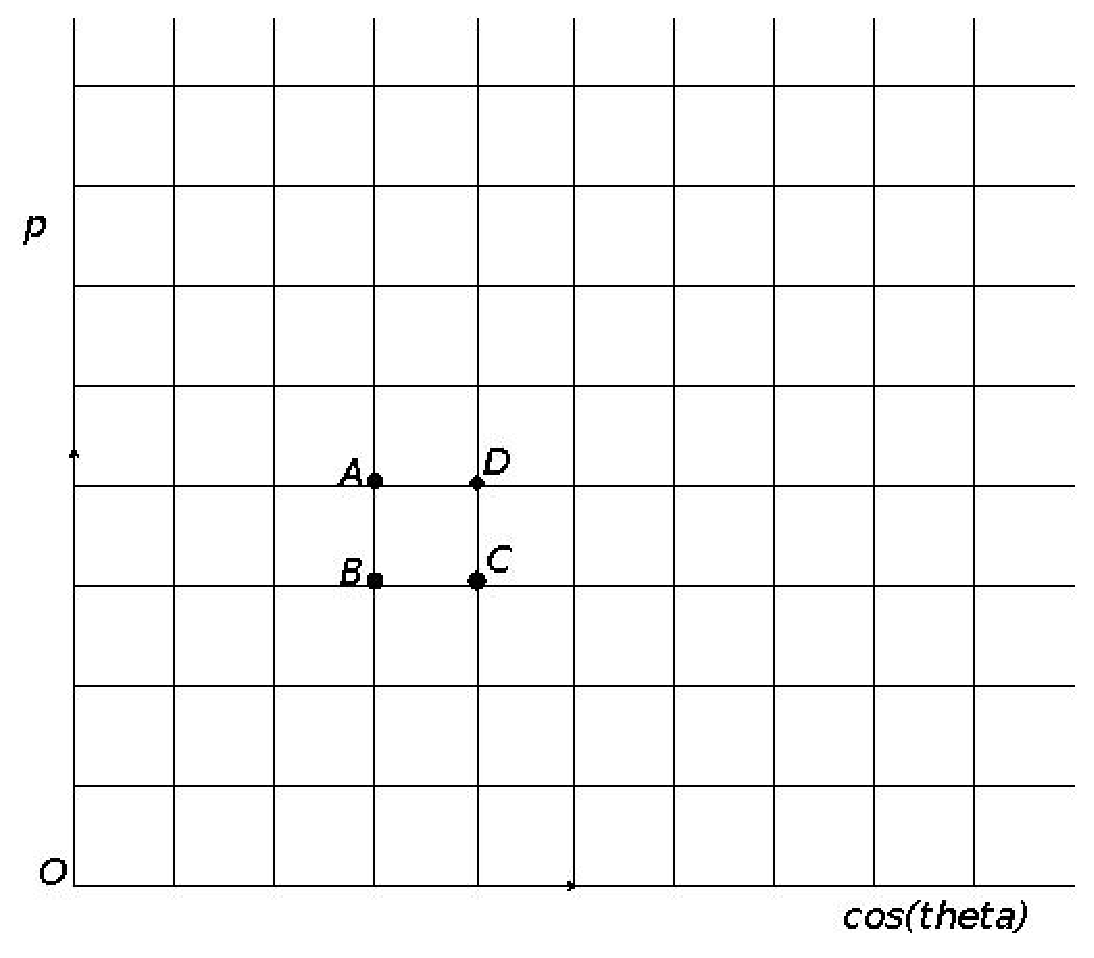
\includegraphics[width=0.6\textwidth]{chap4simul/Figures/kineGrid_steg.eps} 
  \leavevmode \includegraphics[width=0.6\textwidth]{figuresEG4/FigSim/kineGrid_steg.png} 
  \caption[A section of the kinematics grid]{Corners of a typical bin highlighted in the kinematic space covered by the event generator.}
  \label{CSgrid}  %http://wwwold.jlab.org/Hall-B/secure/eg4/adhikari/Simulations/mod_osip_bost_4kpDoc/steg.html
\end{figure}

\begin{comment}
adhikari@ifarm1101> pwd
/w/hallb/claseg4/adhikari/RCSLACPOL/JobSubs/TestExe
adhikari@ifarm1101> m ../stegRcInpFor2_npEb8ms2hSqNw_Eb8F10T0pMax0_000.inp
1.993
-2250
0.01
0.0
0.0
1.0
-100.93
5.000
45.000
250.0
325.0
0.2
1.993
N
N
70000
cs_map.dat
acc_map.dat
steg.bos
2
adhikari@ifarm1101> m ../stegRcInpFor2_npEb7ms2hSqNw_Eb7F30T13pMax0_000.inp 
1.337
-1500
0.01
0.0
0.0
1.0
-100.93
5.000
45.000
250.0
325.0
0.2
1.337
N
N
70000
cs_map.dat
acc_map.dat
steg.bos
2
===============
c Extracting vertex position
      vert_r=rran()*r_beam         ! Vertex radius  kp: 9/18/13: (the third parameter=0.01 in above input file which comes after the torus current)
c+ accordiong e6a target radius=3.5-6 mm
c+ generating outside target volume (on a cylinder surface
c+ but Gagik implemented 1cm radius
c      vert_r = 1.
      vert_phi=rran()*2.e0*pi       ! Vertex phi
      vert_x=x_beam+vert_r*cos(vert_phi)
      vert_y=y_beam+vert_r*sin(vert_phi)
      vert_z=t_offset+(rran()-0.5e0)*t_length  ! Target lenght + offset
======
Looking at the latter parts of steg*.f that was used in the generator, four banks HEAD, MCEV, MCTK & MCVX were used
to produce the BOS files
      CALL BOS(IWW,Nbcs)
      CALL BKFMT('HEAD','I')
      CALL BKFMT('MCEV','I')
      CALL BKFMT('MCTK','(6F,5I)')
      CALL BKFMT('MCVX','(4F,I)')     ! MC vertex parameters
c Booking BOS bank
c general banks
      iHEAD = NBANK('HEAD',0,8,1)  ! BOS HEADER
      IWW(iHEAD+1)=2                ! Version Number
      IWW(iHEAD+2)=RUN              ! Run Number
      IWW(iHEAD+3)=MEVT             ! Event Number
      IWW(iHEAD+4)=0                ! Event Time
      IWW(iHEAD+5)=-1               ! Event Type
      IWW(iHEAD+6)=0                ! ROC: sync status is 0-OK, > 0bit pattern of offending ROC's
      IWW(iHEAD+7)=7                ! Event Classification from DAQ: 1-15 Physics Events
      IWW(iHEAD+8)=1                ! Level 1 Trigger Latch Word (16 bits)
      NR=MEVT
      iMCEV = NBANK('MCEV',0,2,1)
      IWW(iMCEV+1) = int(rran()*100000)  ! first geant random number seed for event
      IWW(iMCEV+2) = int(rran()*100000)  ! second seed
      iMCVX = NBANK('MCVX',0,5,1)
      rw(iMCVX+1) = vert_x         ! x of vertex
      rw(iMCVX+2) = vert_y         ! y
      rw(iMCVX+3) = vert_z         ! z
c      rw(iMCVX+4) = 0e0           ! secs of flight
      rw(iMCVX+4) = 1.e-9*(vert_z-t_offset)/c      ! secs of flight
      IWW(iMCVX+5) = 0              ! vertex flag
c Particle bank
      IMCTK = NBANK('MCTK',0,11,2)
c Electron
      ipart = 11*(1-1)
      rw(imctk+ipart+1)=sin(theta_el)*cos(phi_el) ! x dir cosine at track origin
      rw(imctk+ipart+2)=sin(theta_el)*sin(phi_el) ! y dir cosine
      rw(imctk+ipart+3)=cos(theta_el)             ! z dir cosine
      rw(imctk+ipart+4)=p_el                      ! momentum
      rw(imctk+ipart+5)=me                        ! mass
      rw(imctk+ipart+6)=-1.e0                     ! charge
      IWW(imctk+ipart+7)=11                        ! track Particle Data Group id
      IWW(imctk+ipart+8)=0                         ! track flag
      IWW(imctk+ipart+9)=1                         ! beginning vertex number
      IWW(imctk+ipart+10)=0                        ! ending vertex number
      IWW(imctk+ipart+11)=0                        ! parent track
c Increment event numer
\end{comment}





\subsection{GSIM - CLAS Detector Simulation} 
\label{gsim}
The Monte Carlo events thus generated are next fed into GSIM - the CLAS Monte Carlo simulation program using GEANT 3.21 libraries from CERN \cite{gsimMH_wb}. It %. -which 
simulates the CLAS detector response by implementing a complete model of the detector as well as the propagation of particles through different materials including all physics processes, such as multiple scattering, energy loss, pair production, and nuclear interactions. The program takes the input event particles and then, based on their types, momenta and positions, %then 
``swims'' (traces) them through all %a large number of detector 
volumes of different materials that are defined using various library routines and the detector parameters. Charged particles are also subjected to the effects of the torus and target magnetic fields of the same strength as in the actual experiment (for this the same field maps are used as in the track reconstruction process using RECSIS). All the ingredients of the program (field maps, active detection volumes, passive volumes of detector support structures etc) are modeled as accurately as possible with the help of engineering designs and actual detector measurements. Special subroutines corresponding to various active parts of the detector produce outputs resembling the real detector signals which can then be reconstructed and analyzed just as the real experimental data \cite{clasBrooks}%pg 31 
\cite{bDey_th}. %pg 84
GSIM is configured to match with the conditions of a given experiment by giving it proper values of input parameters via a command line input file which contains various ``ffread cards'' some of which are listed in table-\ref{tab:ffread} along with their values that were used in our simulation.
%thKlimenko: Data Simln pg 86/105, Detector simulation 91/109


%\chapter{FFREAD cards used by GSIM} %Slifer Ap B, pg 205, or Sulkosky 3.2.1 pg 40
\label{ffreadCards}

%\FloatBarrier
% http://tex.stackexchange.com/questions/9485/how-to-fix-table-position
%\begin{center}
\begin{table}[H]%[h!b!p!]
\centering
\caption[FFread cards for GSIM]{Some of the ffread cards \& their values which are used as GSIM input parameters.}
\label{tab:ffread}
    \begin{tabular}{ | l | l |}
    \hline
    \textbf{Cards}      &     \textbf{Values}     \\ \hline
    MAGTYPE     &     2        \\  \hline
    MAGSCALE    &    -0.5829 0.0 \textbf{\textcolor{blue}{(for 1.337 GeV)}}   \\  \hline
    MAGSCALE    &    -0.3886 0.0 \textbf{\textcolor{blue}{(for 1.993 GeV)}}  \\  \hline
    GEOM        &    'ALL'      \\  \hline
    NOMC        &    'EC' 'SC' 'CC' 'DC'      \\  \hline
    NOGEOM      &    'MINI' 'ST'  'TG2' 'TG' 'SOL'      \\  \hline
    NOGEOM      &    'PTG' 'FOIL'      \\  \hline
    NOMATE      &    'PTG' 'FOIL'      \\  \hline
    PTGIFIELD   &     1      \\  \hline
    TMGIFIELD   &     1      \\  \hline
    TMGIFIELDM  &     1      \\  \hline
    TMGFIELDM   &     51.0      \\  \hline
    TMGSCALE    &     0.979       \\  \hline
    PTGMAXRAD   &     300.0      \\  \hline
%    -NTARGET 3
%    -CHAMBER 4
    MGPOS       &    0.0 0.0 -100.93      \\  \hline
    BAFF        &    3. 9. 165.3 9. 180.5 9. 195.8      \\  \hline
    RUNG        &    50556      \\  \hline
    AUTO        &    1       \\  \hline
    KINE        &    1       \\  \hline
    \end{tabular}
%    \caption[FFread cards for GSIM]{Some of the ffread cards \& their values which are used as GSIM input parameters.}
%    \label{tab:ffread}
\end{table}
%\end{center}

\begin{comment}
adhikari@ifarm1101> m ffread10 
CCCUTS .0001 1.e-4 1.e-4 1.e-4 1.e-4
DCCUTS .0001 1.e-4 1.e-4 1.e-4 1.e-4
ECCUTS .0001 1.e-4 1.e-4 1.e-4 1.e-4
ICCUTS .0001 1.e-4 1.e-4 1.e-4 1.e-4
SCCUTS .0001 1.e-4 1.e-4 1.e-4 1.e-4
STCUTS .0001 1.e-4 1.e-4 1.e-4 1.e-4
CUTS   .0001 1.e-4 1.e-4 1.e-4 1.e-4 1.e-4 1.e-4 1.e-4
MAGTYPE 2
MAGSCALE  -0.5829 0.0
GEOM 'ALL'
NOMC 'EC' 'SC' 'CC' 'DC'
NOGEOM 'MINI' 'ST'  'TG2' 'TG' 'SOL'
NOGEOM 'PTG' 'FOIL'
NOMATE 'PTG' 'FOIL'
PTGIFIELD 1
TMGIFIELD 1
TMGIFIELDM 1
TMGFIELDM 51.0
TMGSCALE 0.979 
PTGMAXRAD 300.0
-NTARGET 3
-CHAMBER 4
MGPOS 0.0 0.0 -100.93
BAFF 3. 9. 165.3 9. 180.5 9. 195.8
RUNG 50556
AUTO 1 
KINE 1 
STOP
%
% /u/home/adhikari/SimStuff/SubmitJobs files ffread30/whTcl_0.tcl & ffread10/whTcl_0.tcl for 1.3 & 2.0 GeV simulations
% 
\end{comment}
  %Moved to separate file (SEK suggestion for putting it in appendix, may be worthwile)


\subsection{GSIM POST PROCESSOR (GPP)} 
 \label{gpp}
The GSIM output is next passed onto GPP - another standard %important 
CLAS software package - to process the simulated data further so that the detector response is accounted for more accurately. This package improves the response by smearing the detector signals and removing them if there are dead regions (determined by querying %looking into 
a data base which in turn is made by looking at the raw data of the experiment).
% Look at A. Klimenko's thesis (viewer page 109) (found much better than B. Dey's (page 85)
% Maurizio Ungaru prepared & set up the database for us at the request of M. Ripani

%\begin{comment}  %enable the comment block to disable the following ``red'' comments
%\textbf{\textcolor{red}{Comment: Bring in the file (or some stuff from there) that I wrote on my work on DC-smearing. I may need to shorten the stuff by moving most of the part (describing the work that I did) to either an Appendix or to some separate analysis note. I may give a brief note on how I did that \& only list the numbers that I decided. In addition pay attention to smoothening the logical flow in the introductory part. Avoid redundancy of the statements.}}
%\end{comment}
%\textbf{\textcolor{red}{Heavy editing needs to be done here (old write-up).}}

%%This chapter/section is about the work on ``dc-smearing in GPP''
%Created by kp on Sep 17, 2011

\hspace{0.5cm}
% \newline \newline
%\newline  %double \newline gives underfull warnings

\begin{comment}
This is here just to remind me about this way of making comments
And, also to add some more reminders to myself.
1) change the figure size parameters to fit to the page if possible. 2) if related, put two or more figures side by side to save space as well as to make the organization better (otherwise, the compiler may put figures randomly and thus losing the sense of order/continuity)

It is assumed that the efficiency depends on the number of photoelectrons (the corresponding variable in the data ntuple is ``nphe''), which in turn is determined by the hit location on the Cerenkov PMT-projected plane (defined by the projected 
\th and \ph) as well as the angle with which the particle hit the plane. \ref{fig:genEvnts3}
\end{comment}

%%%%%%%%%%%%%%%%%%%
%   Note: The following section disabled because it is also in introChp4Sim.tex which includes this file with \input{filename}
%%%%%%%%%%%%%%%%%%%
%\section{GSIM POST PROCESSOR (GPP)}  
A lot of known, unknown, quantified, and unquantified factors such as temperature, alignment, dead channels, electronic malfunction etc affect the performance of the CLAS detector. But, GSIM does not include all these effects and, hence, the efficiency of the detector is always less than what the simulation provides us. To make the simulation more realistic by taking into account some of those effects, another CLAS software called GSIM Post Processor (GPP) is used to process the GSIM output. The GPP can change the DC, SC, CC and EC signals produced in the simulation. The DC signals can be changed by (a) accounting for the dead wires according to the calibration database, (b) shifting the DOCA mean value, and (3) smearing the hit signals according to the resolution determined by the calibration database or according to the command line input. Likewise, SC signals can be changed with a parameter input for smearing the time resolution. And, for the CC and EC signals, the GPP can use the hardware thresholds\cite{jxZhang_th}.

As the experimental conditions and detector configurations can change from one experiment to another, in order to run the GPP, we must have our own experiment specific calibration constants and parameters such as the run number (R), the DC smearing scale values for regions 1, 2 and 3 (a, b, c) and the SC smearing scale value (f). Even for a given experiment, these constants and parameters are determined to be different for different data sets (corresponding to a given beam energy, for example). The value for R can be any run number belonging to a specific data set. This number is used to identify the entry of the calibration constants in the database that corresponds to the given data set.  In order to simplify the job, we decided to use the timing resolutions determined by the calibration database assuming that they are good enough and need only to determine new values for the DC smearing. %(the reason to do this is that with the default (calibration database) resolution, the energy resolution in the data and the simulation seemed to differ significantly (as will be evident below when we compare the widths of the simulation & real data elastic peaks) 
To further simplify the job, we assumed that the three DC Regions had identical resolutions, so the DC smear parameters a, b, and c would have the same values, and the common DC-smear value is what is determined from the procedure described below.



%\subsection{\href{http://www.jlab.org/Hall-B/secure/eg4/adhikari/Analysis/SimStuffs/moniDcSmear.html}{Determining Dc-smear scales for GPP} to have the energy resolution of simulation comparable with that of the CLAS}
In order to determine the DC-smear, we generated a statistically significant number (about half million) of elastic-electron events distributed according to the elastic cross section and then ran them through GSIM, GPP and RECSIS. The pure proton target events, turning off the radiative effects are generated using the existing %Genova inherited 
STEG event generator. %As an example, the 2.3 GeV events looked like as shown in fig(\ref{fig:genEvnts3}) when histogrammed in the quantity $\Delta$E.

%(/w/hallb/claseg4/adhikari/GSIM_RECSIS/mod_osip_bost/mod_osip_bostVadim11_64tNH3). I modified the two files sgm_model.f & cor_peak_proton.f 
%which are kept for backup in the same directory where eps files are. In addition, the routines of bost.f were replaced with the latest 
%(/w/hallb/claseg4/adhikari/GSIM_RECSIS/bost09.f, soft linked by the old name bost.f), both generate_map and work directories use all these three files
% See my comments on cor_peak_proton.f at the very bottom of this file
\begin{comment} %Disabling this one to replace it with a figure that his a caption on the side rather than at the bottom.
\begin{figure}[h] %ht, htpb (p - float, b = bottom, h=? t = top)
  \leavevmode 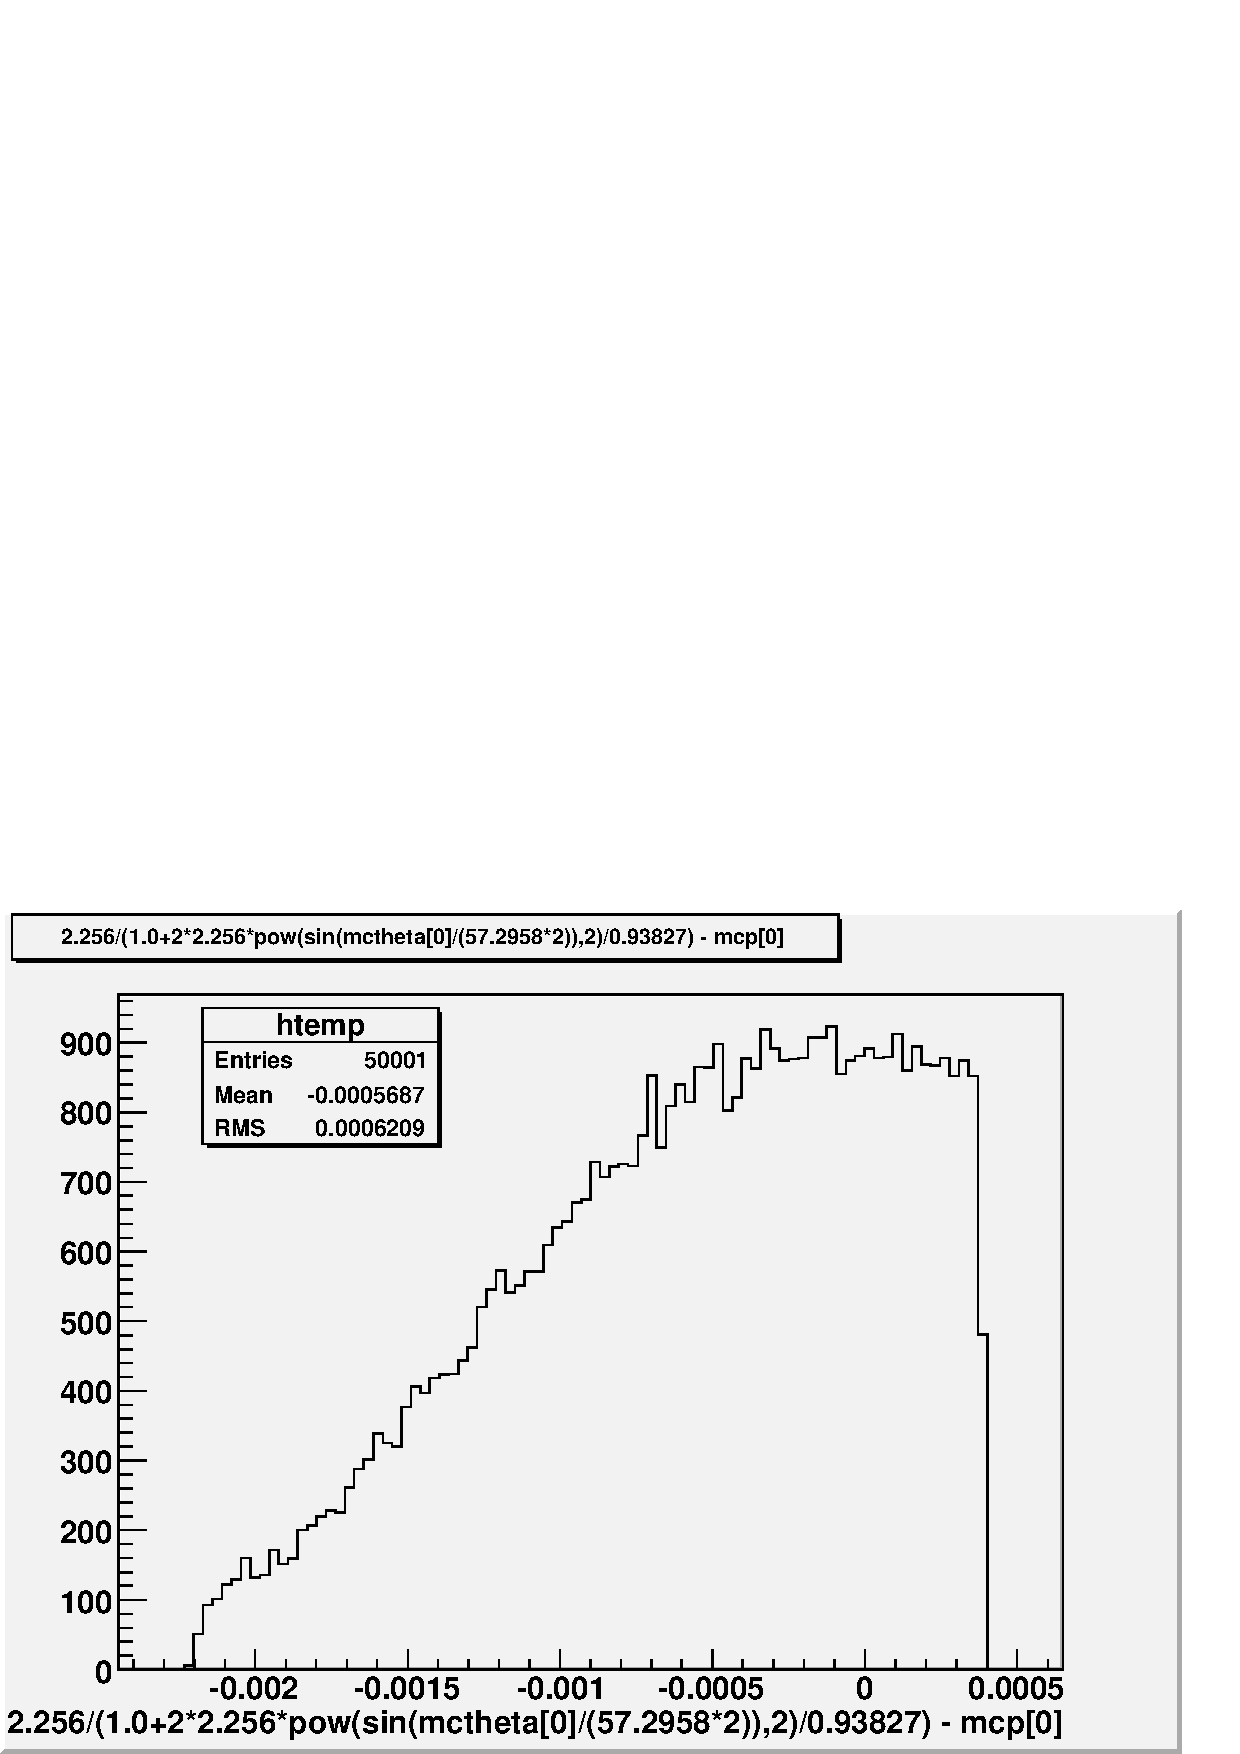
\includegraphics[width=0.6\textwidth]{figuresEG4/DcSmear/genEvntsElastOnlyEb3.png} 
  \caption[$\Delta$E of generated elastic events]{$\Delta$E of 2.3 GeV generated elastic-only proton-target events (no internal radiative effects).}
  \label{fig:genEvnts3}
\end{figure}



\begin{SCfigure} %http://en.wikibooks.org/wiki/LaTeX/Floats,_Figures_and_Captions (needs packages \usepackage[pdftex]{graphicx} & \usepackage{sidecap})
  \centering
  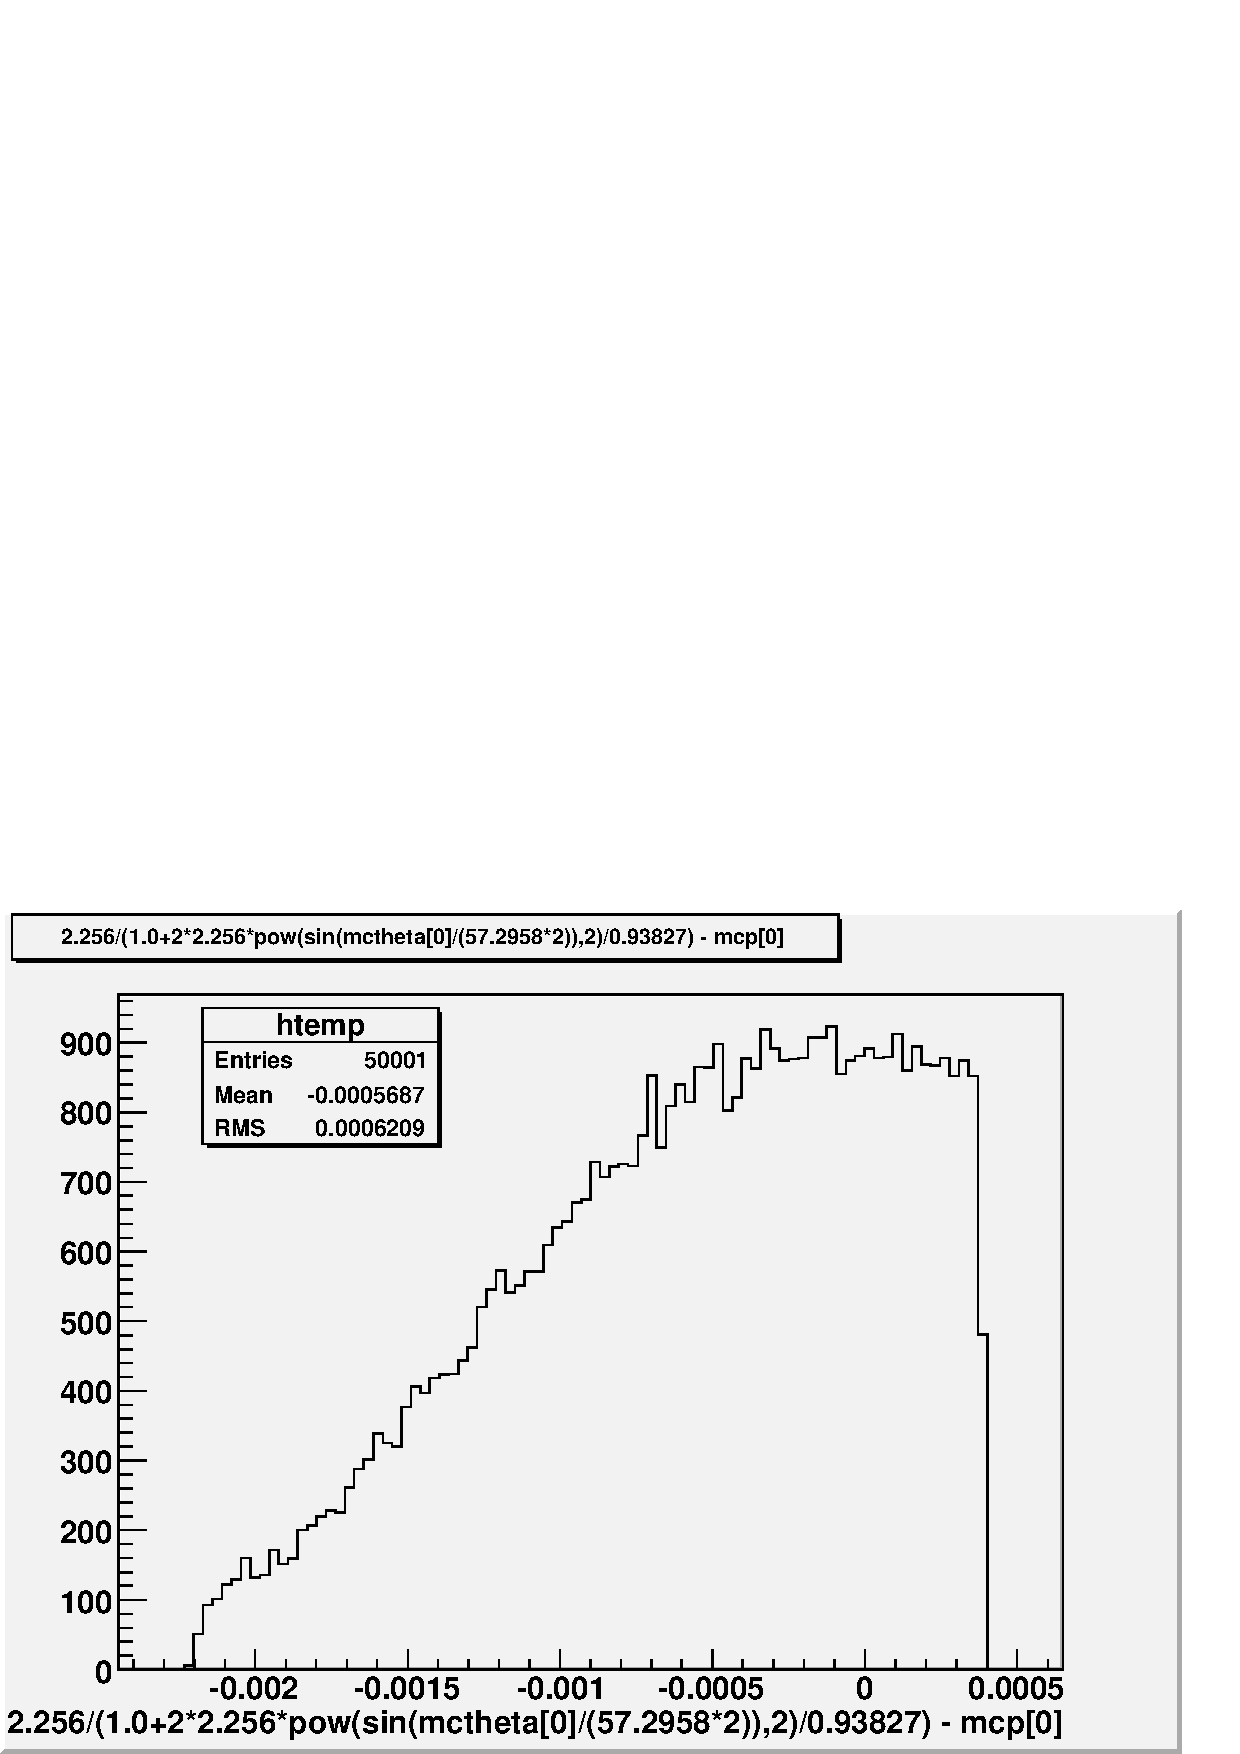
\includegraphics[width=0.7\textwidth]{figuresEG4/DcSmear/genEvntsElastOnlyEb3.png}
  \caption[$\Delta$E of generated elastic events]{$\Delta$E of 2.3 GeV generated elastic-only proton-target events (no internal radiative effects).}
  \label{fig:genEvnts3}
\end{SCfigure}

 \end{comment}

%\subsection{Finding the variation of the width of the simulated elastic peak as a function of DC-smear scale for GPP.}
The simulated elastic events are then fed into GSIM, GPP and RECSIS, with GSIM and RECSIS used in the same configuration as when processing the CLAS data 
during the ``pass-1'' phase, and GPP run with different values of DC-smear scales as inputs. The reconstructed data coming out of RECSIS corresponding to 
a given value of DC-smear is then histogrammed in $\Delta$E again and fitted to a Gaussian to get its $\sigma$ (characterizing width) of and mean 
(characterizing position). As we can see in figures \ref{fig:dcSm1.3} and \ref{fig:dcSm2.9}, %fig(\ref{fig:dcSmEff}), %This didn't give proper number
the width of the elastic peak increases with the DC-smear but the position stays more or less the same as expected. In fact, when the two are plotted 
against DC-smear (as in figures \ref{fig:SigmaVsm} and \ref{fig:MeanVsm}) %(as in fig (\ref{fig:ParsVsm})), %This didn't give proper number 
the width shows a linear dependance.



%Don't delete the following commented out lines. They are important reminders.
%The following four images are made using ~/Acceptance/SimStuffs/dE_resolHistoFits.C and enabling ``#define DRAW_EPS'' & ``#define USE_THETA_ALL''
\begin{comment} %=======================================Comments begin
%idea source: http://texblog.wordpress.com/2007/08/01/placing-figurestables-side-by-side-minipage/ : Placing figures/tables side-by-side (\minipage)
%This method of putting figures/tables side by side doesn't have the option of global caption (if there is, it treats it like a
% caption of a different figure assigning it with a different figure number in the output file. So, I chose the 'subfigure' method instead
\begin{figure}[h]
\begin{minipage}[b]{0.5\linewidth}
\centering
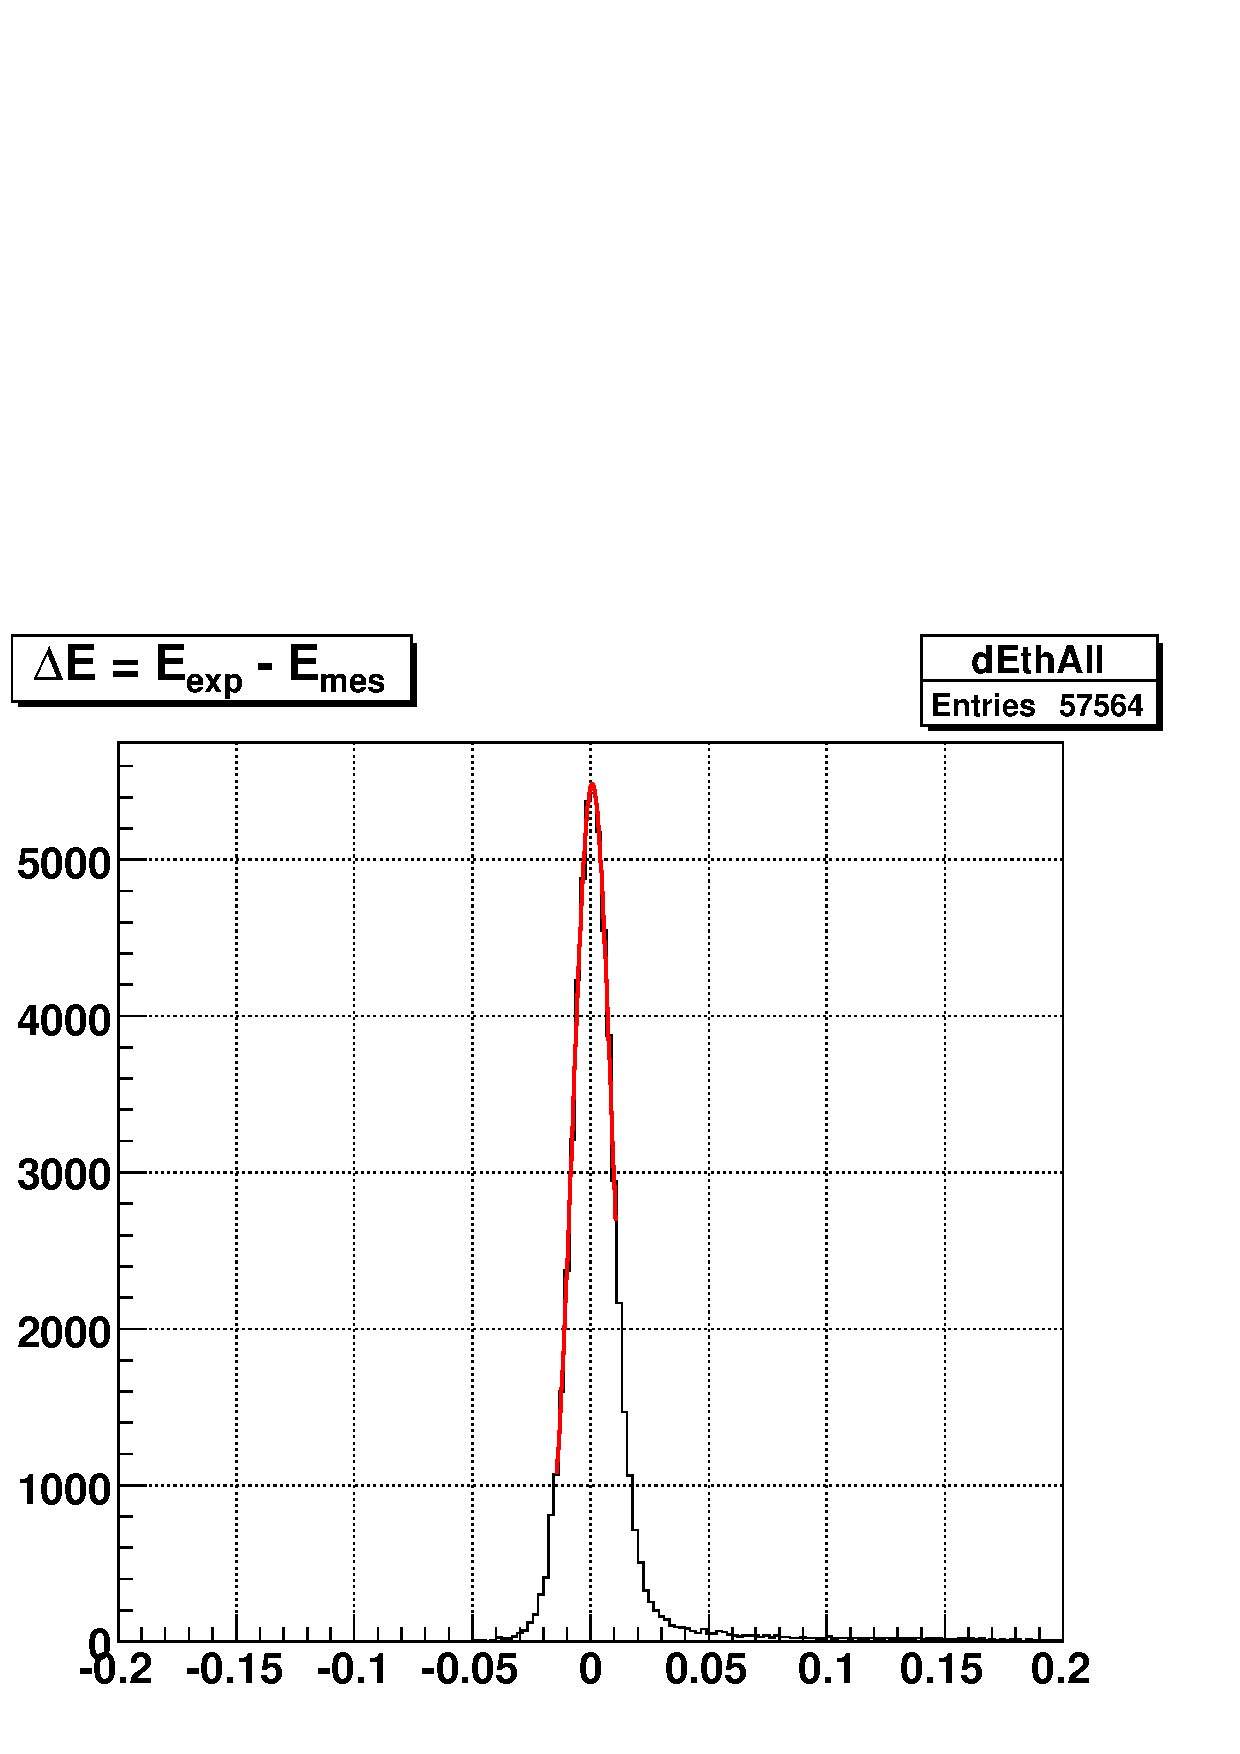
\includegraphics[scale=0.37]{figuresEG4/DcSmear/dE_ThAllEb3_DcSmear1.3.png}
\caption{$\Delta$E of 2.3 GeV simulated elastic-only proton-target events (see fig(\ref{fig:genEvnts3})) after passing through GSIM, GPP 
  (with Dc-smear scale of 1.3) and RECSIS.}
\label{fig:figure1}
\end{minipage}
\hspace{0.0cm} %\hspace{0.1cm}
\begin{minipage}[b]{0.5\linewidth}
\centering
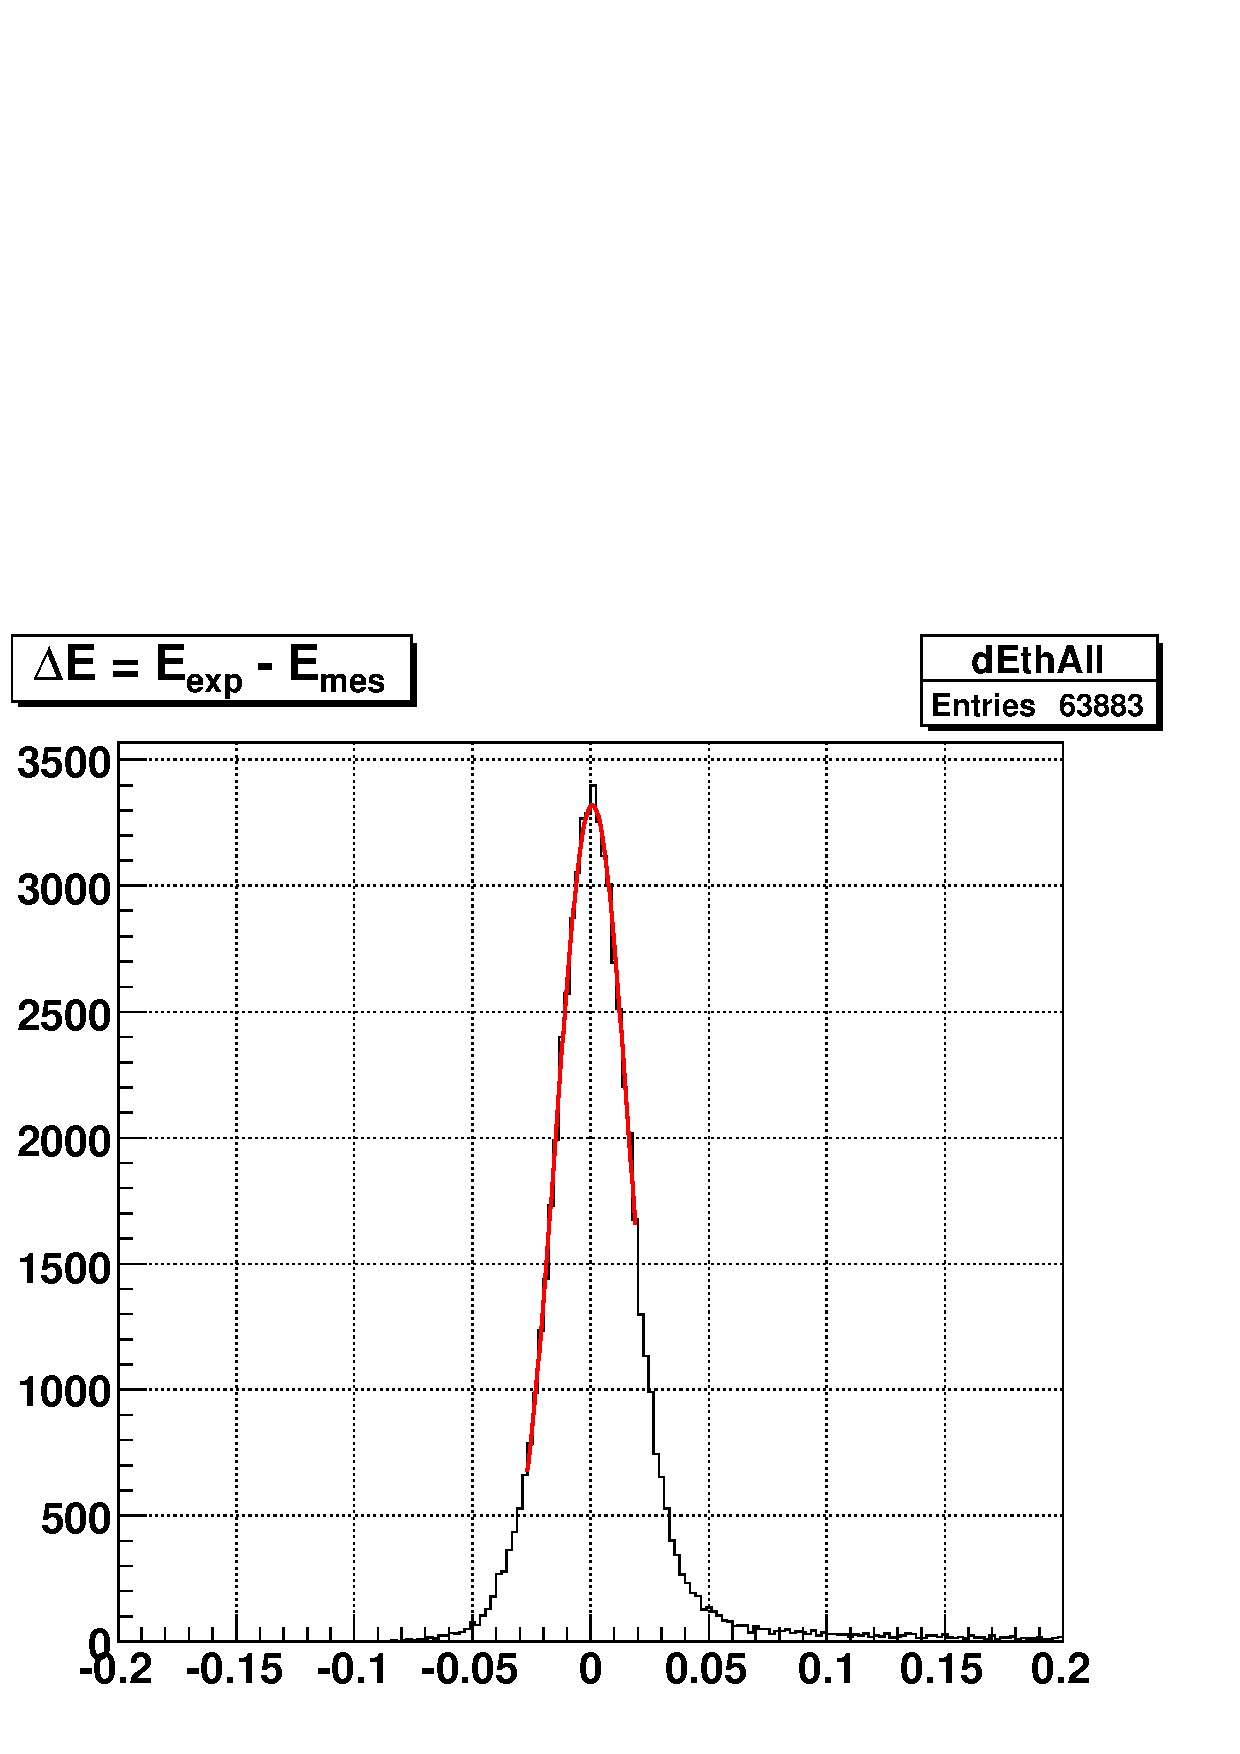
\includegraphics[scale=0.37]{figuresEG4/DcSmear/dE_ThAllEb3_DcSmear2.9.png}
\caption{$\Delta$E of 2.3 GeV simulated proton elastic-only events after passing through GSIM, GPP (with Dc-smear scale of 2.9) and RECSIS.}
\label{fig:figure2}
\end{minipage}
\caption{$\Delta$E of 2.3 GeV simulated elastic-only proton-target events (see fig(\ref{fig:genEvnts3})) after passing through GSIM, GPP (with Dc-smear scale of 1.3) and RECSIS.}
\end{figure}
\end{comment}  %=======================================Comments end


% idea source: http://texblog.wordpress.com/2007/08/28/placing-figurestables-side-by-side-subfigure/ :Placing figures/tables side-by-side (\subfigure)
% Can include any number of figures/tables, not just two.
\begin{figure}[H]
\centering
\subfigure[Dc-smear]{
\includegraphics[scale=0.32]{figuresEG4/DcSmear/dE_ThAllEb3_DcSmear1p3}%.png}
\label{fig:dcSm1.3}
}
\subfigure[Dc-smear]{
\includegraphics[scale=0.32]{figuresEG4/DcSmear/dE_ThAllEb3_DcSmear2p9}%.png}
\label{fig:dcSm2.9}
}
\label{fig:dcSmEff} %Effect of Dc-smear
%\caption[Optional caption for list of figures]{Caption of subfigures \subref{fig:subfig1}, \subref{fig:subfig2} and \subref{fig:subfig3}}
\caption[$\Delta$E of reconstructed simulated events]{$\Delta$E of 2.3 GeV simulated elastic-only proton-target events passing through GSIM, GPP (with two different Dc-smear scales), and RECSIS.}
\end{figure}




\begin{figure}[H]
\centering
\subfigure[$\sigma$ vs DC-smear]{
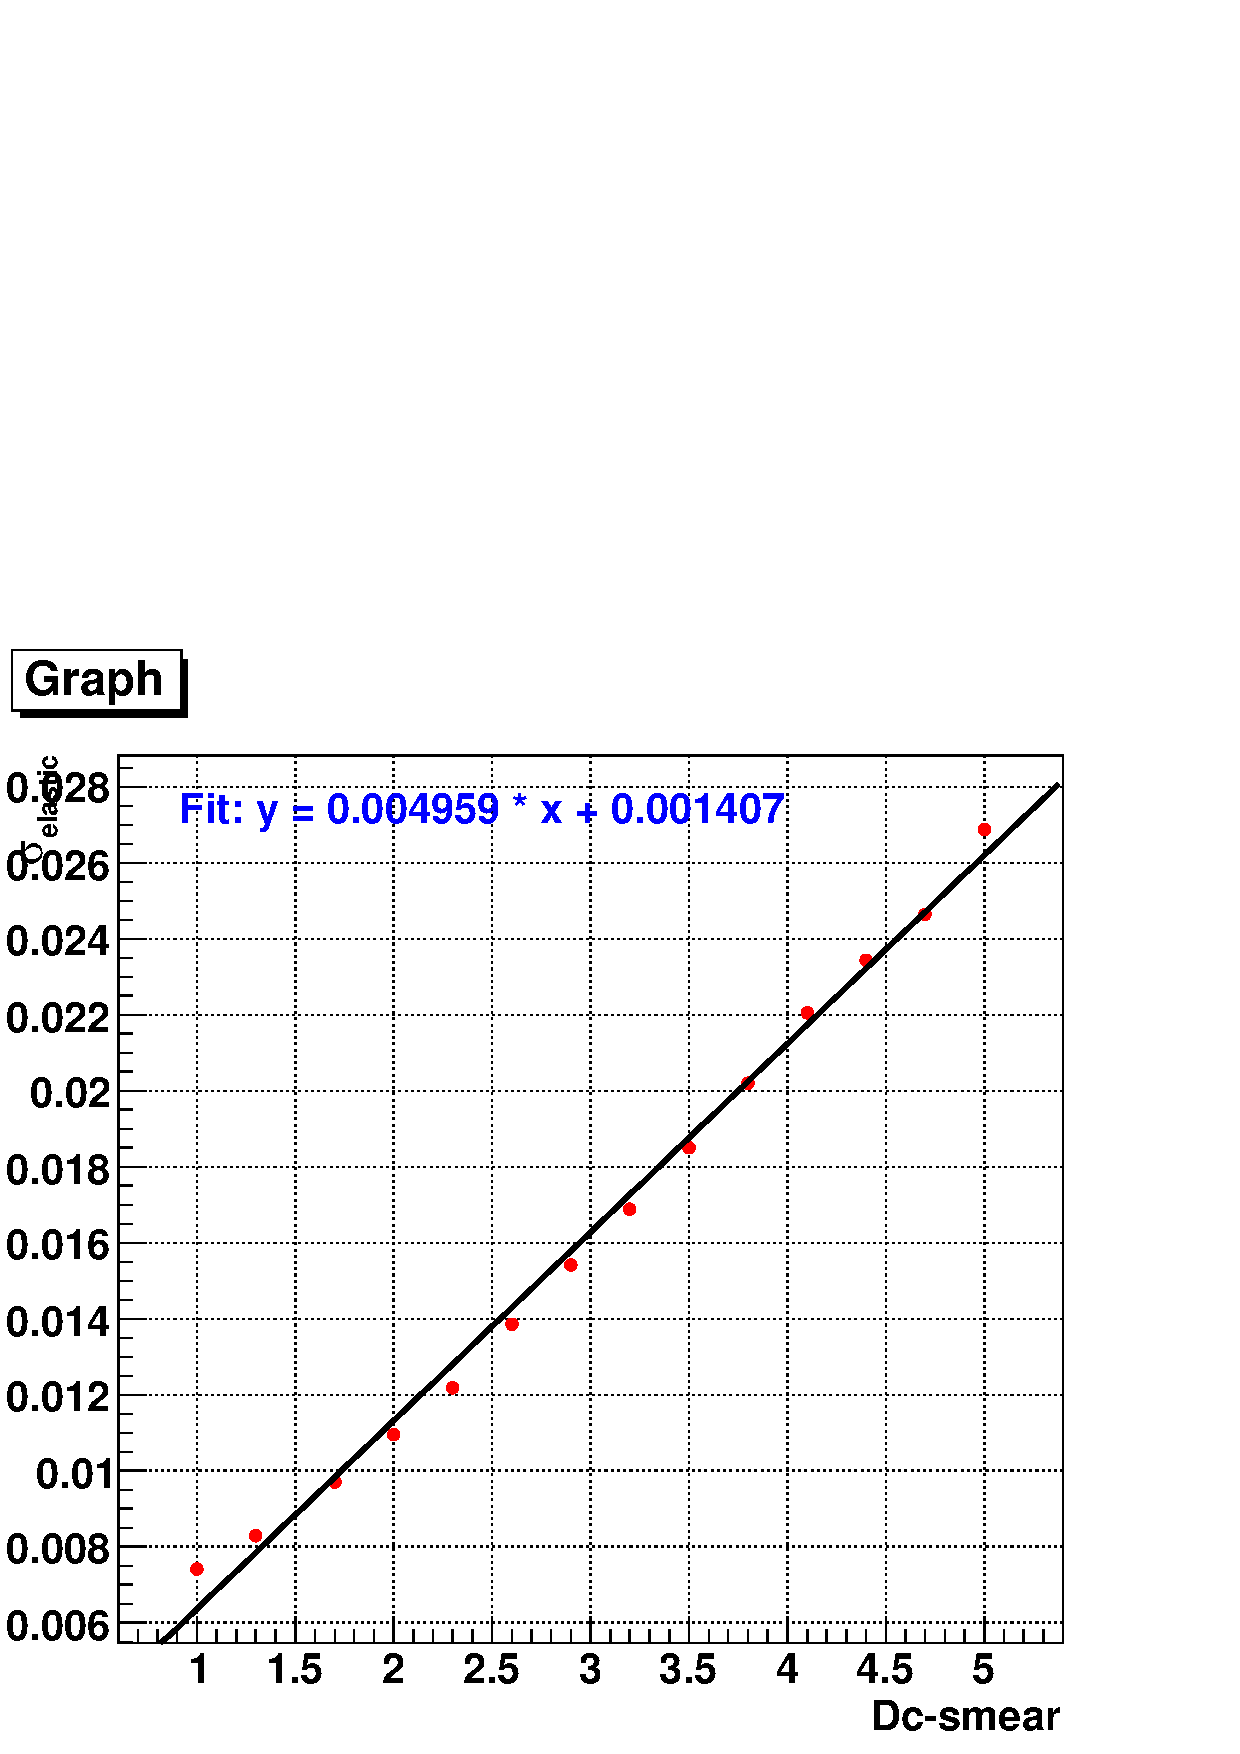
\includegraphics[scale=0.32]{figuresEG4/DcSmear/grSigmaVsDcSmear_Eb3.png}
\label{fig:SigmaVsm}
}
\subfigure[Mean vs DC-smear]{
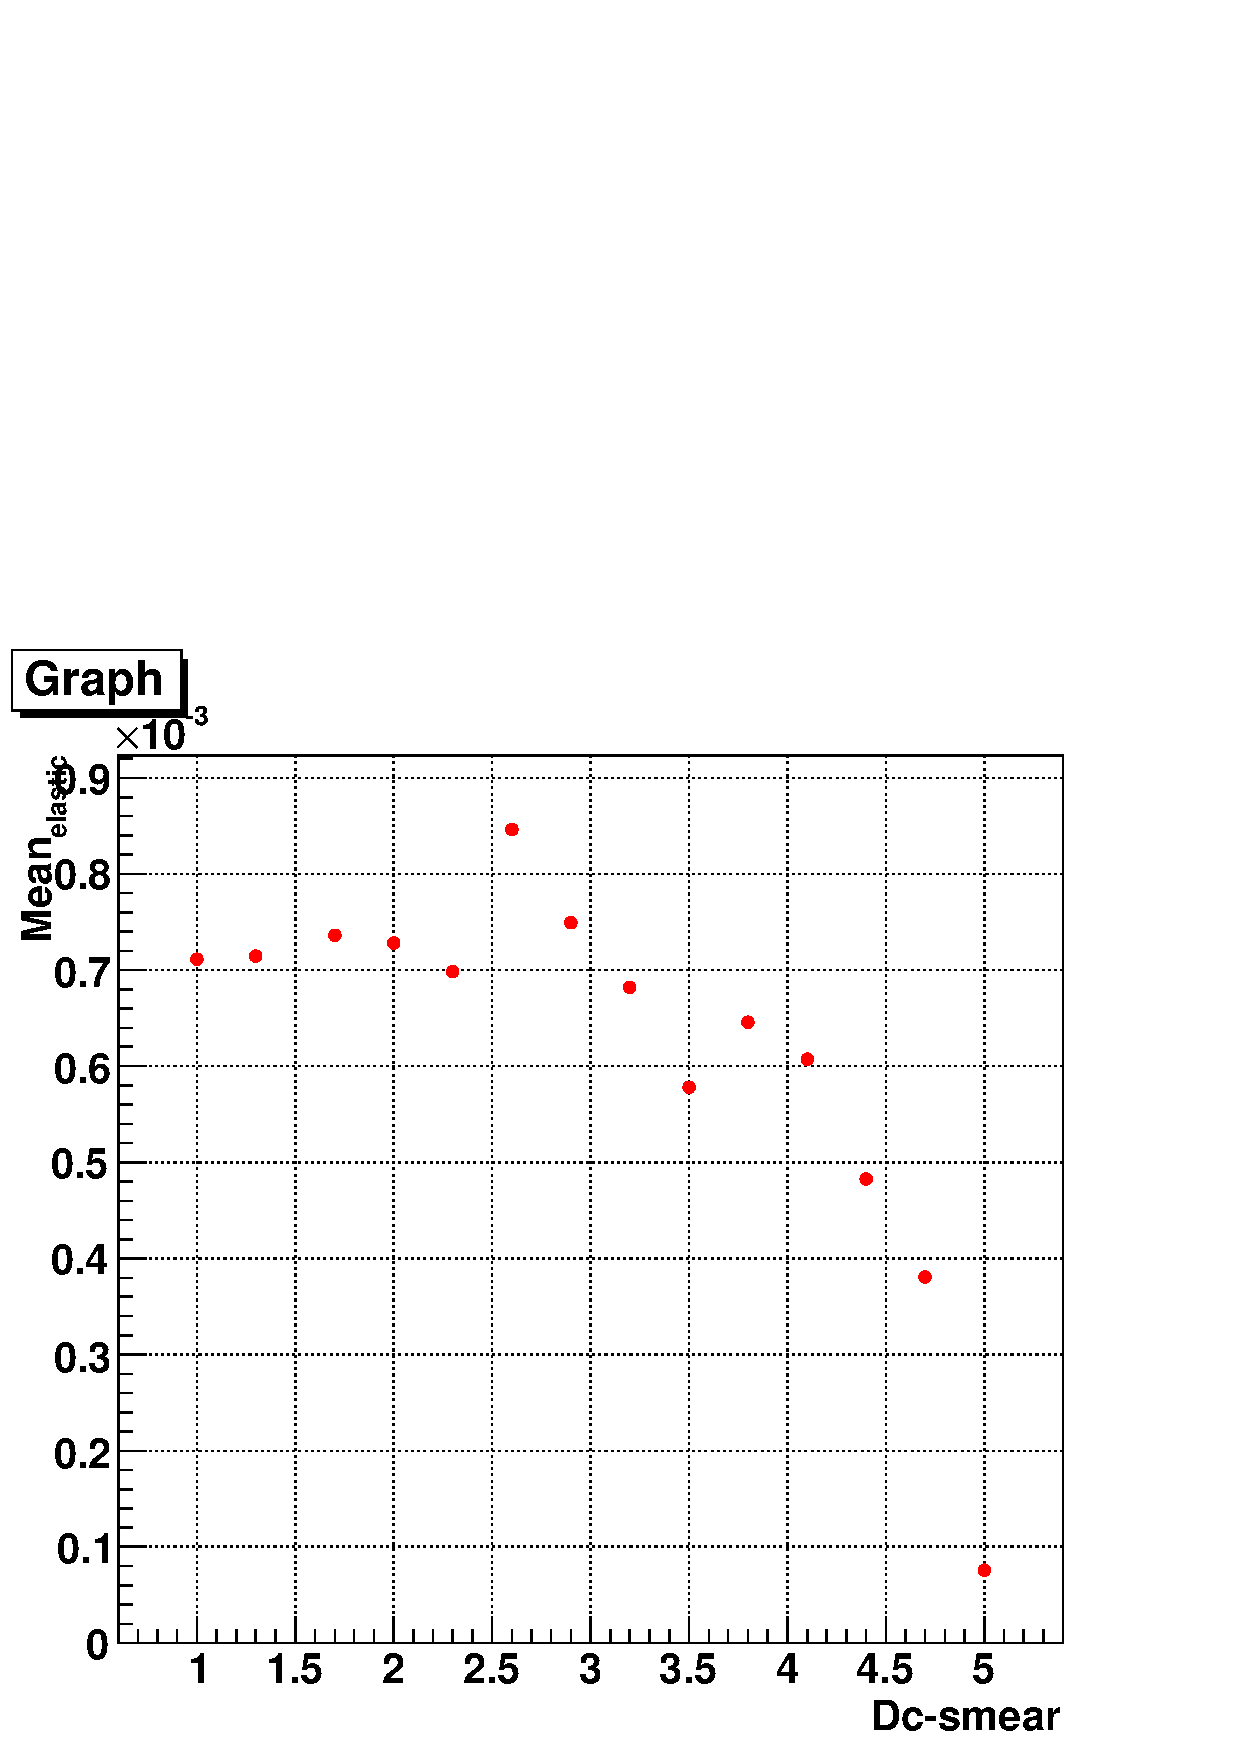
\includegraphics[scale=0.32]{figuresEG4/DcSmear/grMeanVsDcSmear_Eb3.png}
\label{fig:MeanVsm}
}
\label{fig:ParsVsm} %Effect of Dc-smear
%\caption[Optional caption for list of figures]{Caption of subfigures \subref{fig:subfig1}, \subref{fig:subfig2} and \subref{fig:subfig3}}
\caption[DC-smearing effects on elastic peak]{Graphs showing the dependence of width and position (obtained from the Gaussian fits as shown in the fig (\ref{fig:dcSmEff}) of the elastic peaks on the DC-smear applied to GPP.}
\end{figure}


\subsection{Finding the width of the real CLAS data elastic peak.}
With the knowledge of the DC-smear dependence of energy resolution (Fig. \ref{fig:SigmaVsm}), if we also know the resolution in the real data, 
we can determine the right value of DC-smear which would make the resolution in the simulation comparable with that in the real data. So, 
the next step is to find the resolution in the real CLAS data, which is done again by measuring the width of the elastic peak in the real data. 
But, because the real data is a very complex mixture of events coming from various reaction channels, we must first have a way to separate the elastic 
data from the rest. One method entails histogramming \dE from both the \nh3 and \c12 target data (for a given beam energy) and subtracting 
the latter (after the cross-normalization) from the former (as in fig (\ref{fig:elNH3mC})) to effectively remove the contribution from nitrogen 
component of the \nh3 target leaving the contribution coming only (mostly) 
%More words about this background subtraction can be found in the section for the inclusive momentum correction.
from the proton component. Another method consists of using only the \nh3 data but this time calculating the helicity dependent cross-section 
difference in the elastic region Fig. (\ref{fig:elXsDif}). In the latter method, the difference removes the contribution from the unpolarized 
nuclear background because they have the same contribution to the opposite helicity state cross-sections. After the elastic data is separated, its 
\dE distribution is fitted to a Gaussian as with the simulation data and we arrive at the experimental energy resolution. 
%Since on the simulation side, we used the total cross-section, to make an apple-to-apple comparison, the measurement coming from the 1st method
%would be better choice for the experimental data.

% Put a intra-thesis chapter/section link (rather than the web link) in thesis version
% \href{http://www.jlab.org/Hall-B/secure/eg4/ripani/Reference/Reference.html}{groups 1, 2 and 4 cuts}. 
% Check DoEvent..() function in file /u/home/adhikari/Acceptance/SimStuffs/dE_resol_DataSim.C to see what cuts were used to select the events


%The following image is made using ~/Acceptance/SimStuffs/subtractHistos4ProdElast.C and enabling ``#define DRAW_EPS'' & ``#define USE_THETA_ALL''
%The following four images are made using ~/Acceptance/SimStuffs/dE_resolHistoFits.C and enabling ``#define DRAW_EPS'' & ``#define USE_THETA_ALL''
\begin{figure}[h] %ht, htpb (p - float, b = bottom, h=? t = top)
\centering
  \leavevmode 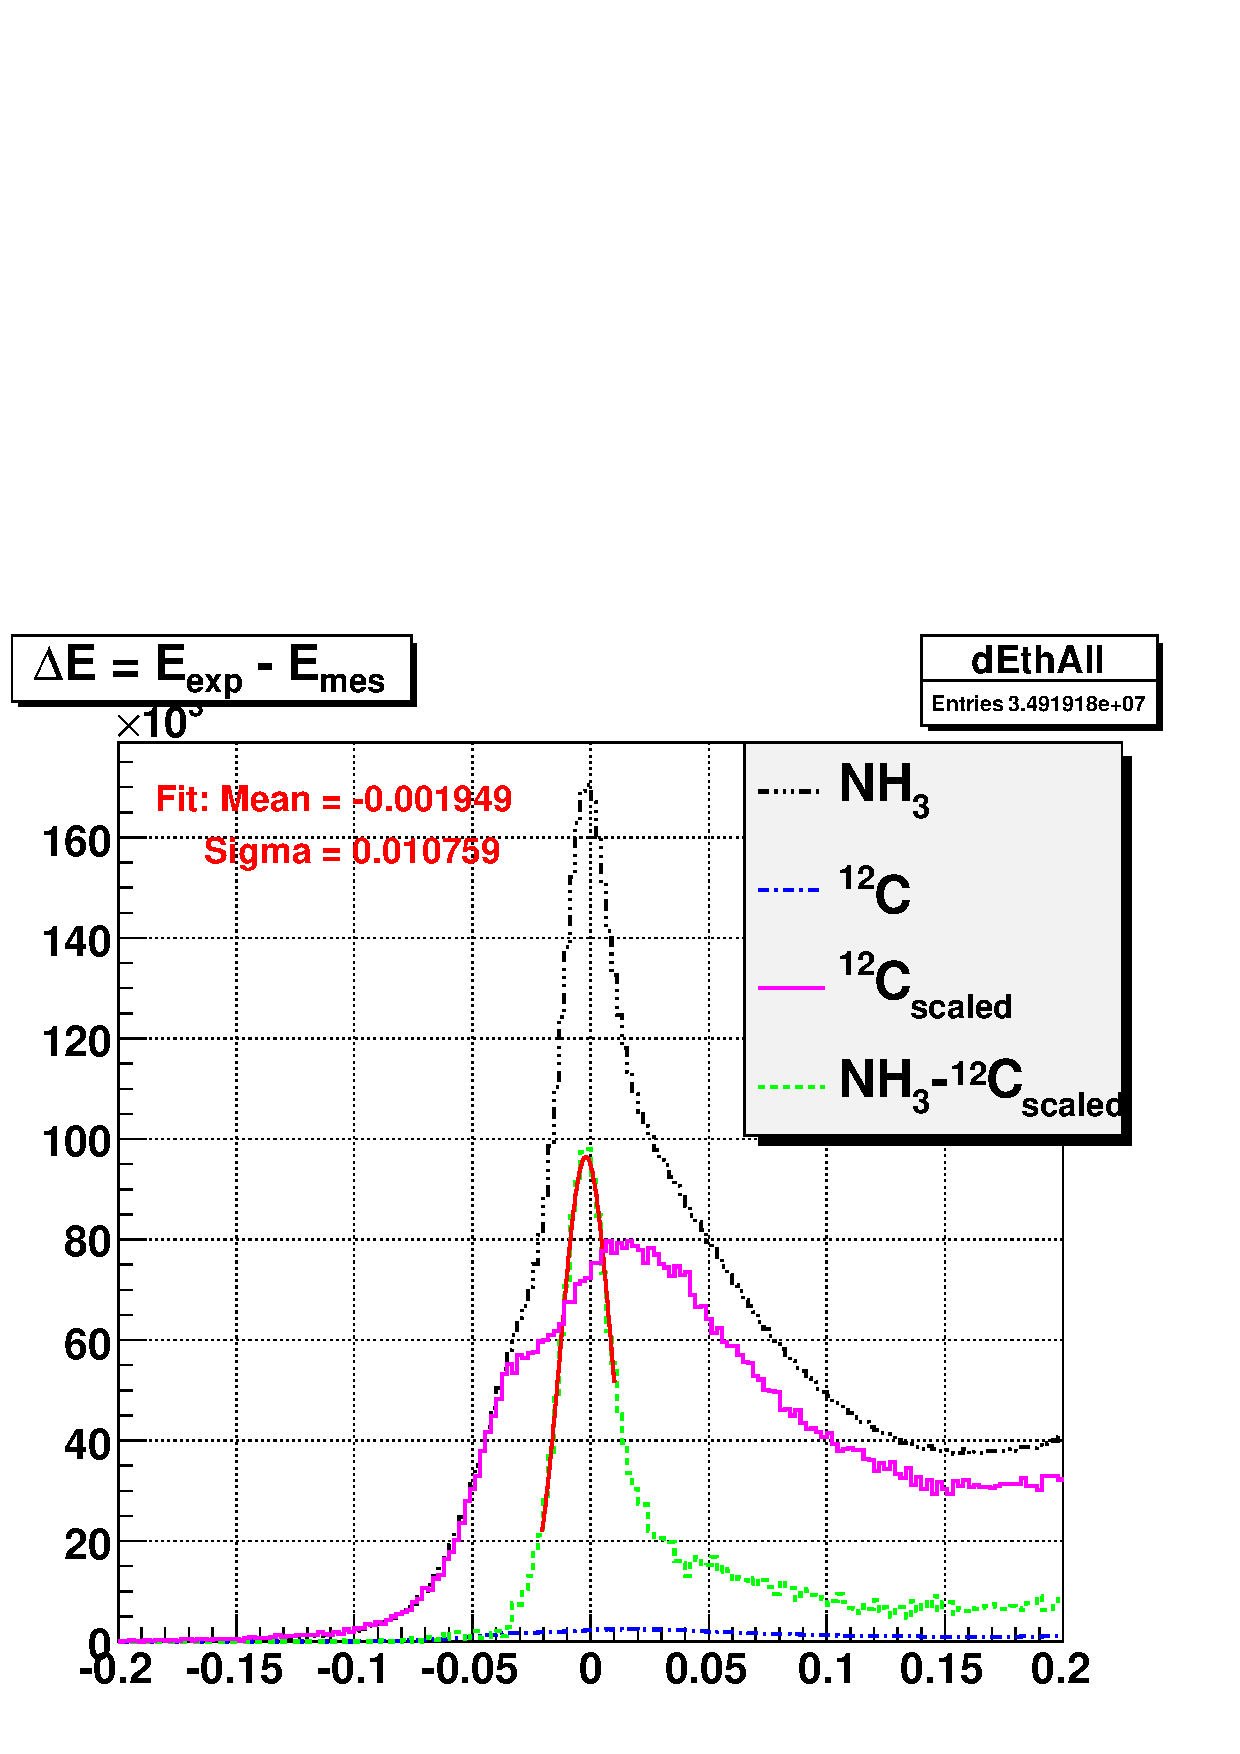
\includegraphics[width=0.8\textwidth]{figuresEG4/DcSmear/dE_elastProdEb3.png} 
  \caption[Background subtraction to get elastic peak]{Histograms illustrating the extraction of elastic peak for 2.3 GeV by using carbon-12 data for background removal from the total-cross section (all good electrons with $\theta>7$ used).}
  \label{fig:elNH3mC}
\end{figure}

%The following image is made using ~/Acceptance/SimStuffs/subtractHistos4xsDiff.C and enabling ``#define DRAW_EPS'' & ``#define USE_THETA_ALL''
\begin{figure}[h] %ht, htpb (p - float, b = bottom, h=? t = top)
\centering
  \leavevmode 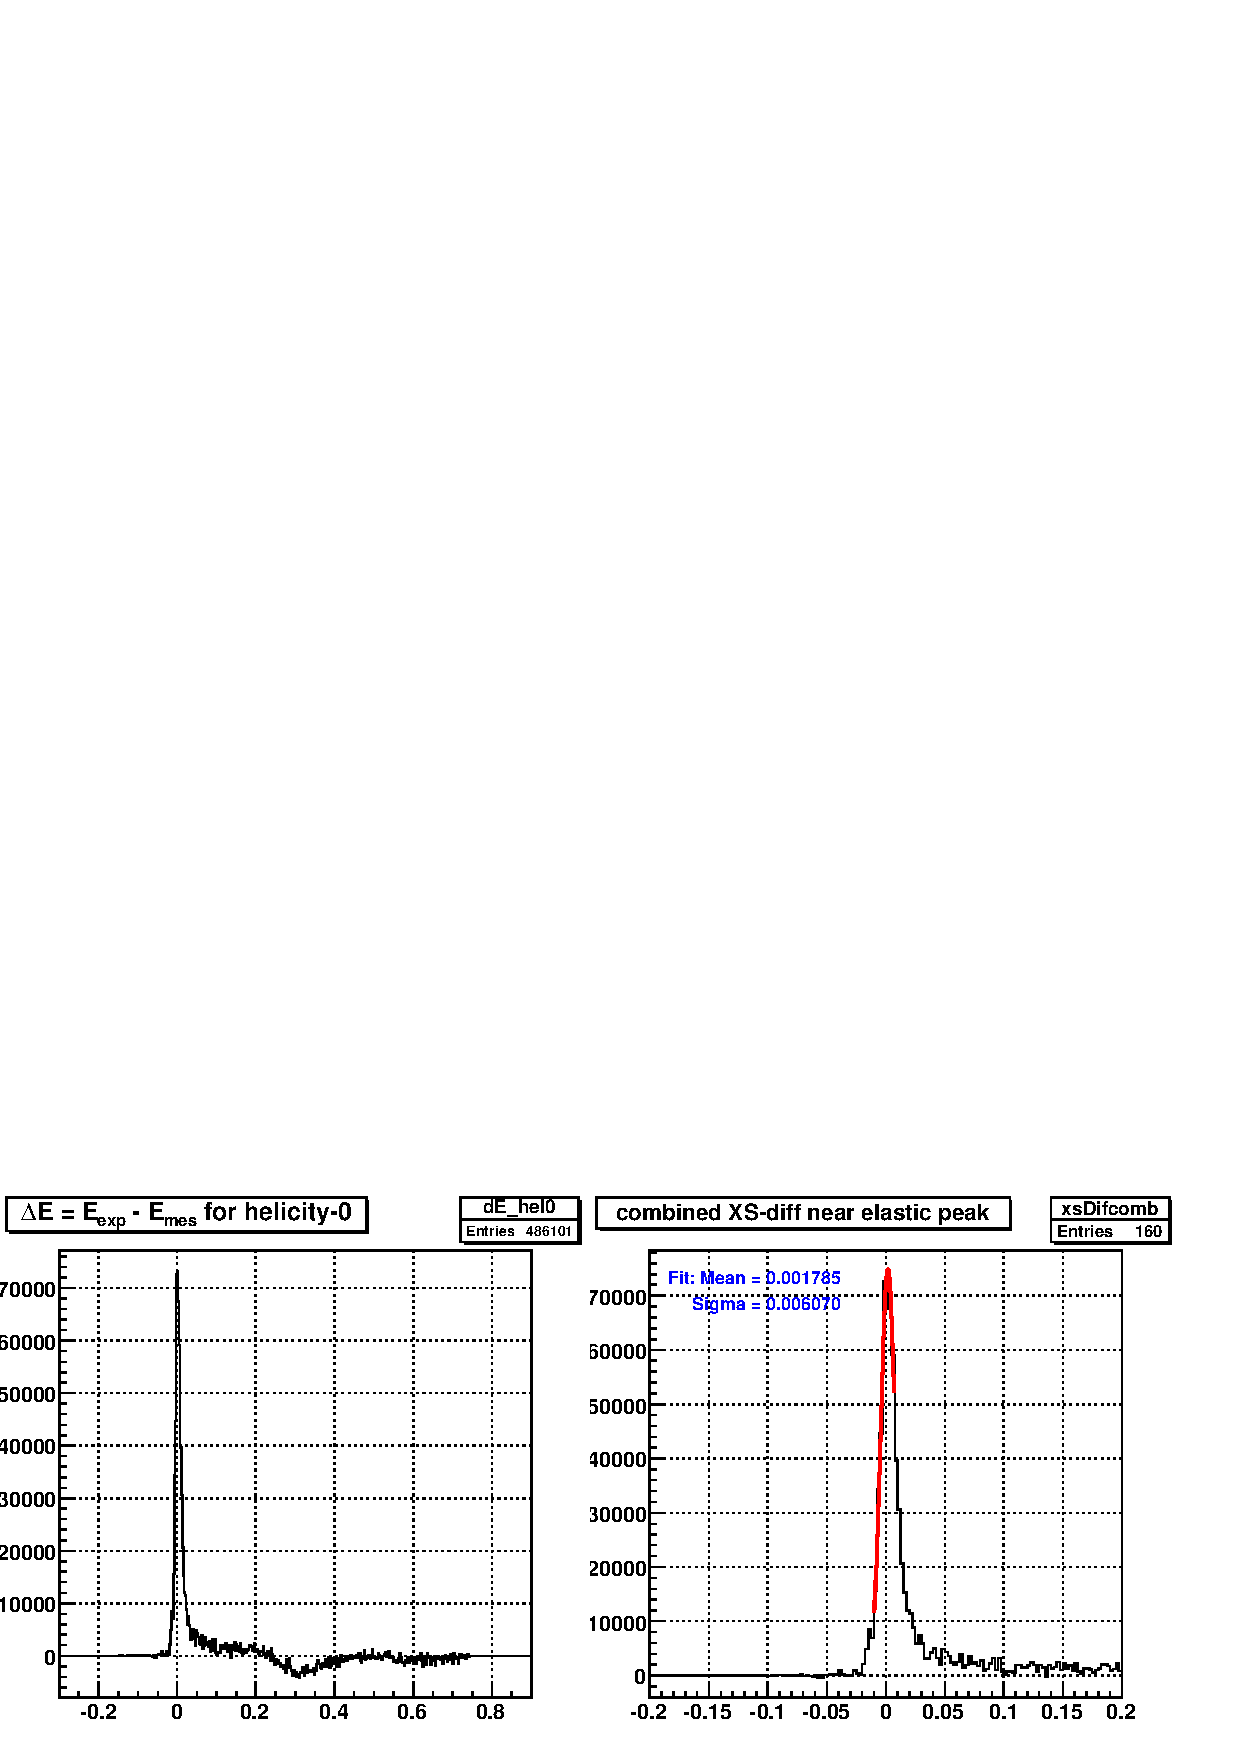
\includegraphics[width=1.0\textwidth]{figuresEG4/DcSmear/dE_elastXsDiffEb0Tgt11.png} 
  \caption[Cross-section difference]{Plots showing the cross-section difference for 2.3 GeV NH$_3$ target data with the right one zoomed in around the elastic region (all good electrons with $\theta>7$ used).}
  \label{fig:elXsDif}
\end{figure}

 %\\ %12/4/13 (Addressing Gabriel's concern)
 %\\
 



%\subsection{Comparing the width of the real CLAS data elastic peak and those from Simulation with different DC-smears.}
%The following two images are made using ~/Acceptance/SimStuffs/graphSigmaVsEb.C and enabling ``#define DRAW_EPS'' & ``#define USE_THETA_ALL''
Using the first of the two methods mentioned above, the real data resolutions were evaluated for three different %cases 
polar angle ($\theta$) cuts - 
all \th (in fact $\theta\ge7^o$), $\theta>15^o$, and $\theta>20^o$. The dependence of these experimental resolutions on the beam energy for these cases are 
shown together in the Fig. \ref{fig:sigsProd}, along with the resolution for the case ``all $\theta$'', but determined from the cross-section difference 
method. Likewise, as described above, the DC-smear dependence of the simulated resolution were determined separately for all these three cases of 
angle cuts, so that we could compare the experimental resolutions with the simulations correspondingly. One such comparison is illustrated in 
the figure \ref{fig:sigsProdSim}, where we show resolutions evaluated for the case of ``all \th'' - first two for the experimental data and the rest for 
the simulated data. 

    
     
 \begin{figure}[h] %ht, htpb (p - float, b = bottom, h=? t = top)
\centering
  \leavevmode \includegraphics[width=1.0\textwidth]{figuresEG4/DcSmear/graphSigmaVsEb_prodOnly.png} 
  \caption[$E_{beam}$ dependence of DC smearing (Experimental) ]{Graphs showing the dependence of width ($\sigma$) of the elastic peaks (from experimental data) on the beam energy (GeV).}
  \label{fig:sigsProd}
\end{figure}
    
 \begin{figure}[h] %ht, htpb (p - float, b = bottom, h=? t = top)
\centering
  \leavevmode 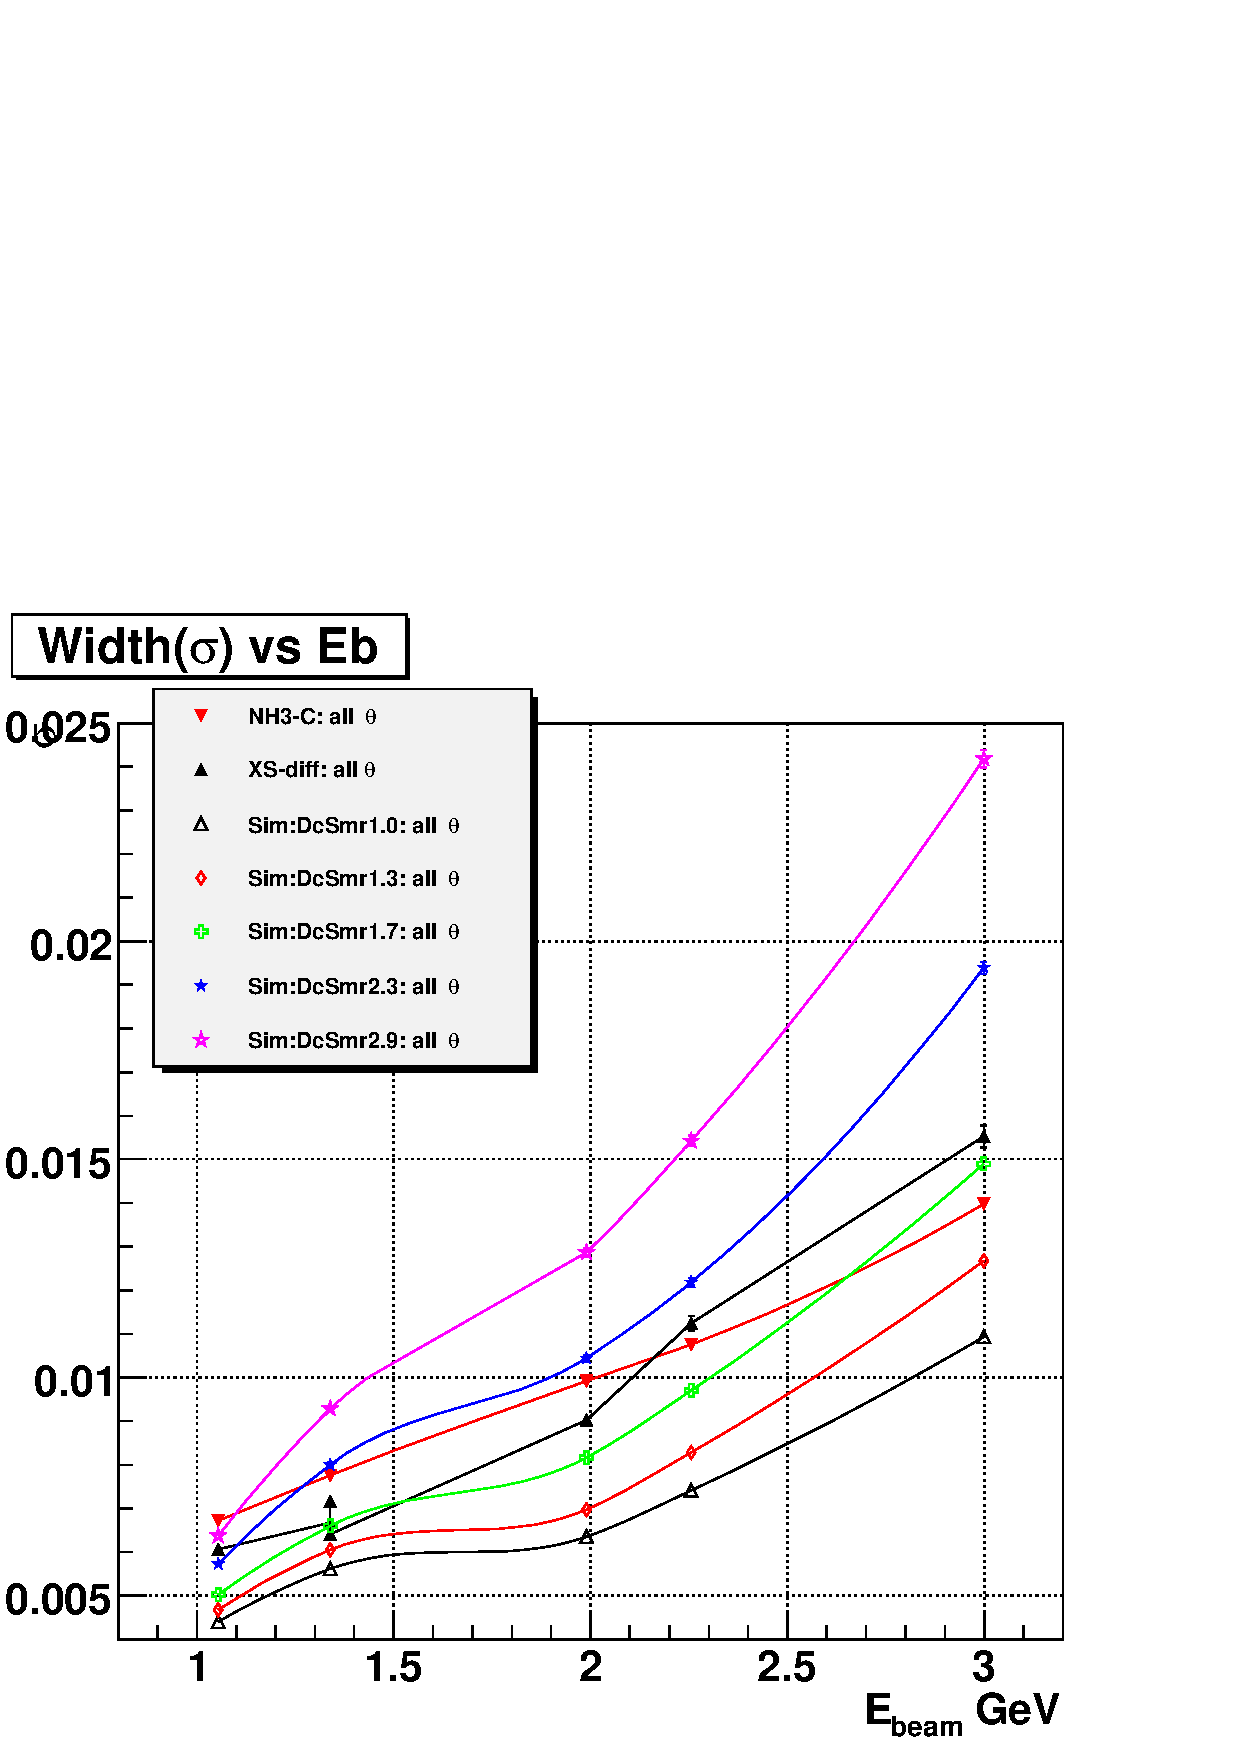
\includegraphics[width=1.0\textwidth]{figuresEG4/DcSmear/graphSigmaVsEb_SimThAll.png} 
  \caption[$E_{beam}$ dependence of DC smearing (Experimental) ]{Graphs showing the dependence of width ($\sigma$) of the elastic peaks (from both experimental and simulated data) on the beam energy (GeV).}
  \label{fig:sigsProdSim}
\end{figure}
    
     
     
Looking at Fig. \ref{fig:sigsProd}, it is obvious that the resolution is $\theta$-dependent as expected. %Remember resol = beta/sqrt(p_t), mom-cor
When the experimental and simulated resolutions are compared for the three different cases of $\theta$ cuts, we realize that the GPP asks for the 
\th dependent DC-smearing, which makes the simulation work very complicated with the current version of GPP. To simplify the situation, we decide to 
have a global (\th independent) value of DC-smearing (for a given beam energy) by comparing the experimental and simulated resolutions corresponding to 
the case of ``all \th'' cut. %That should be good enough for practical purposes. %xz:
%xz: "That should be good enough for practical purposes". Why?  Be careful to never make a statement without backing it up.
By taking into account the fact that there seems to be an inherent 
uncertainty in the measurement of the resolutions (evident from the discrepancy of the experimental resolutions determined from the two different methods)
and comparing the experimental and simulated results, the values as listed in Table. \ref{tab:dcSmears} are chosen for the DC-smearing scales for the GPP.


%\FloatBarrier  
% \FloatBarrier %http://tex.stackexchange.com/questions/9485/how-to-fix-table-position
%\begin{center}
\begin{table}[H]%[h] %[h!b!p!]
\centering
    \caption{DC-smearing scales determined for different beam energies.}
    \label{tab:dcSmears}
    \begin{tabular}{ | l | l | l | l | l | l |}
    \hline
    $E_{beam}$ (GeV) & 1.054  & 1.339 & 1.989 & 2.256 & 2.999 \\ \hline
    DC-smear         & 2.6    & 2.0   & 2.0   & 2.0   & 1.7 \\  \hline
    \end{tabular}
%    \caption{DC-smearing scales determined for different beam energies.}
%    \label{tab:dcSmears}
\end{table}
%\end{center}




\begin{comment} %==================My comments on the generated events==========Comments begin=== Sep 19, 2011
%The events were generated by using the Genova inherited mod_osip_bost (aka STEG) generator 
      subroutine smrad_proton(Es,theta,Ep,sig_el,sig_tot,sel,smin)
      common/material/TG
      sn2=(sin(theta/2.0))**2     Q2=4.0*Es*Ep*sn2       nu=Es-Ep
c-----input values
      Mp=0.93827        Z=1      A=1     E3=Es/(1.0+Es*(1.0-cos(theta))/Mp)
c-----elastic peak width==resolution
      dWp=0.001       delta_E=(dWp+dWp**2/(2.0*Mp))/(1.0+2.0*Es/Mp*sn2)/5.
c-----Target thickness
      t=0.0181              ! 0.6 cm NH3
      tiw=0.0079            ! 7.45 mm He
      tfw=0.0079            ! 7.45 mm He

      elra=0.0d+0       innn=0.0d+0       eltail=0.0d+0
c-----cross section
      if(Ep.gt.(E3-2.0*delta_E)) then
      varr=abs(nu-Q2/(2.0*Mp))
      jack=Es/E3
      elcor=elasrad_proton(Es,theta,t,delta_E,Z,A,tiw,tfw)                     ! cole smith program for radiative correction in the elastic region
      elra=sig_elastic_proton(Es,theta,Mp,Z)*elcor*peak_proton(varr,dWp)*jack
      
      innn=0.0d+0
      eltail=0.0d+0
      else
      elra=0.0d+0
      
      streg_tail=straggling_elasic_proton(Z,Mp,t,Es,Ep,theta,delta_E)           !But this is not added to anything so it's inconsequencial
      endif
            
      sel=elra+eltail
      smin=elra+innn+eltail
      return
      END


Comments:
There are two if blocks in the above chunk of the code:
     a) the ``if'' block which covers the elastic region
     b) the  ``else'' block which covers the rest of the region.
The else block has zero contribution to the value returned by the function because we set 'innn' and 'eltail' to zero and 'streg_tail' is not added to 
the sum to be returned.

As we see, the way I did is (being unsure how to turn off the effect of elcor (Cole smith's rad-corr)) leave the target widths t, tiw and tfw as they 
were (i.e. to non-zero values), and also leave the elcor factor alone, so that it would have some modulating effect on the remaining part of the product  
i.e. sig_elastic_proton(Es,theta,Mp,Z)*peak_proton(varr,dWp)*jack. Initially I thought I would give elcor an artificial value of 1.0 and that would 
probably turn off the effect. But, because of lack of confidence in that idea, I abandoned that idea and left it to modulate the elastic peak (may be 
the peak would come out more like a Gaussian, if I had done that). Even with that modulation, the generated events are within 3 MeV range and so the 
modulation would be insignificant. Another thought that came to my mind was that since this factor should have the effect of reducing the events in the 
elastic region to compensate for the radiative tail that we get beyond the elastic region, and since we're not simulating that part, there is no point 
in worrying about that reduction. If if the factor reduced the cross-section, the generator would produce the same number of events by running some extra 
mile to compensate for that reduction. 
\end{comment}  %=======================================Comments end

%%%%%%%%%%This chapter/section is about the work on ``dc-smearing in GPP''
%Created by kp on Sep 17, 2011

\hspace{0.5cm}
% \newline \newline
%\newline  %double \newline gives underfull warnings

\begin{comment}
This is here just to remind me about this way of making comments
And, also to add some more reminders to myself.
1) change the figure size parameters to fit to the page if possible. 2) if related, put two or more figures side by side to save space as well as to make the organization better (otherwise, the compiler may put figures randomly and thus losing the sense of order/continuity)

It is assumed that the efficiency depends on the number of photoelectrons (the corresponding variable in the data ntuple is ``nphe''), which in turn is determined by the hit location on the Cerenkov PMT-projected plane (defined by the projected 
\th and \ph) as well as the angle with which the particle hit the plane. \ref{fig:genEvnts3}
\end{comment}

%%%%%%%%%%%%%%%%%%%
%   Note: The following section disabled because it is also in introChp4Sim.tex which includes this file with \input{filename}
%%%%%%%%%%%%%%%%%%%
%\section{GSIM POST PROCESSOR (GPP)}  
A lot of known, unknown, quantified, and unquantified factors such as temperature, alignment, dead channels, electronic malfunction etc affect the performance of the CLAS detector. But, GSIM does not include all these effects and, hence, the efficiency of the detector is always less than what the simulation provides us. To make the simulation more realistic by taking into account some of those effects, another CLAS software called GSIM Post Processor (GPP) is used to process the GSIM output. The GPP can change the DC, SC, CC and EC signals produced in the simulation. The DC signals can be changed by (a) accounting for the dead wires according to the calibration database, (b) shifting the DOCA mean value, and (3) smearing the hit signals according to the resolution determined by the calibration database or according to the command line input. Likewise, SC signals can be changed with a parameter input for smearing the time resolution. And, for the CC and EC signals, the GPP can use the hardware thresholds\cite{jxZhang_th}.

As the experimental conditions and detector configurations can change from one experiment to another, in order to run the GPP, we must have our own experiment specific calibration constants and parameters such as the run number (R), the DC smearing scale values for regions 1, 2 and 3 (a, b, c) and the SC smearing scale value (f). Even for a given experiment, these constants and parameters are determined to be different for different data sets (corresponding to a given beam energy, for example). The value for R can be any run number belonging to a specific data set. This number is used to identify the entry of the calibration constants in the database that corresponds to the given data set.  In order to simplify the job, we decided to use the timing resolutions determined by the calibration database assuming that they are good enough and need only to determine new values for the DC smearing. %(the reason to do this is that with the default (calibration database) resolution, the energy resolution in the data and the simulation seemed to differ significantly (as will be evident below when we compare the widths of the simulation & real data elastic peaks) 
To further simplify the job, we assumed that the three DC Regions had identical resolutions, so the DC smear parameters a, b, and c would have the same values, and the common DC-smear value is what is determined from the procedure described below.



%\subsection{\href{http://www.jlab.org/Hall-B/secure/eg4/adhikari/Analysis/SimStuffs/moniDcSmear.html}{Determining Dc-smear scales for GPP} to have the energy resolution of simulation comparable with that of the CLAS}
In order to determine the DC-smear, we generated a statistically significant number (about half million) of elastic-electron events distributed according to the elastic cross section and then ran them through GSIM, GPP and RECSIS. The pure proton target events, turning off the radiative effects are generated using the existing %Genova inherited 
STEG event generator. %As an example, the 2.3 GeV events looked like as shown in fig(\ref{fig:genEvnts3}) when histogrammed in the quantity $\Delta$E.

%(/w/hallb/claseg4/adhikari/GSIM_RECSIS/mod_osip_bost/mod_osip_bostVadim11_64tNH3). I modified the two files sgm_model.f & cor_peak_proton.f 
%which are kept for backup in the same directory where eps files are. In addition, the routines of bost.f were replaced with the latest 
%(/w/hallb/claseg4/adhikari/GSIM_RECSIS/bost09.f, soft linked by the old name bost.f), both generate_map and work directories use all these three files
% See my comments on cor_peak_proton.f at the very bottom of this file
\begin{comment} %Disabling this one to replace it with a figure that his a caption on the side rather than at the bottom.
\begin{figure}[h] %ht, htpb (p - float, b = bottom, h=? t = top)
  \leavevmode 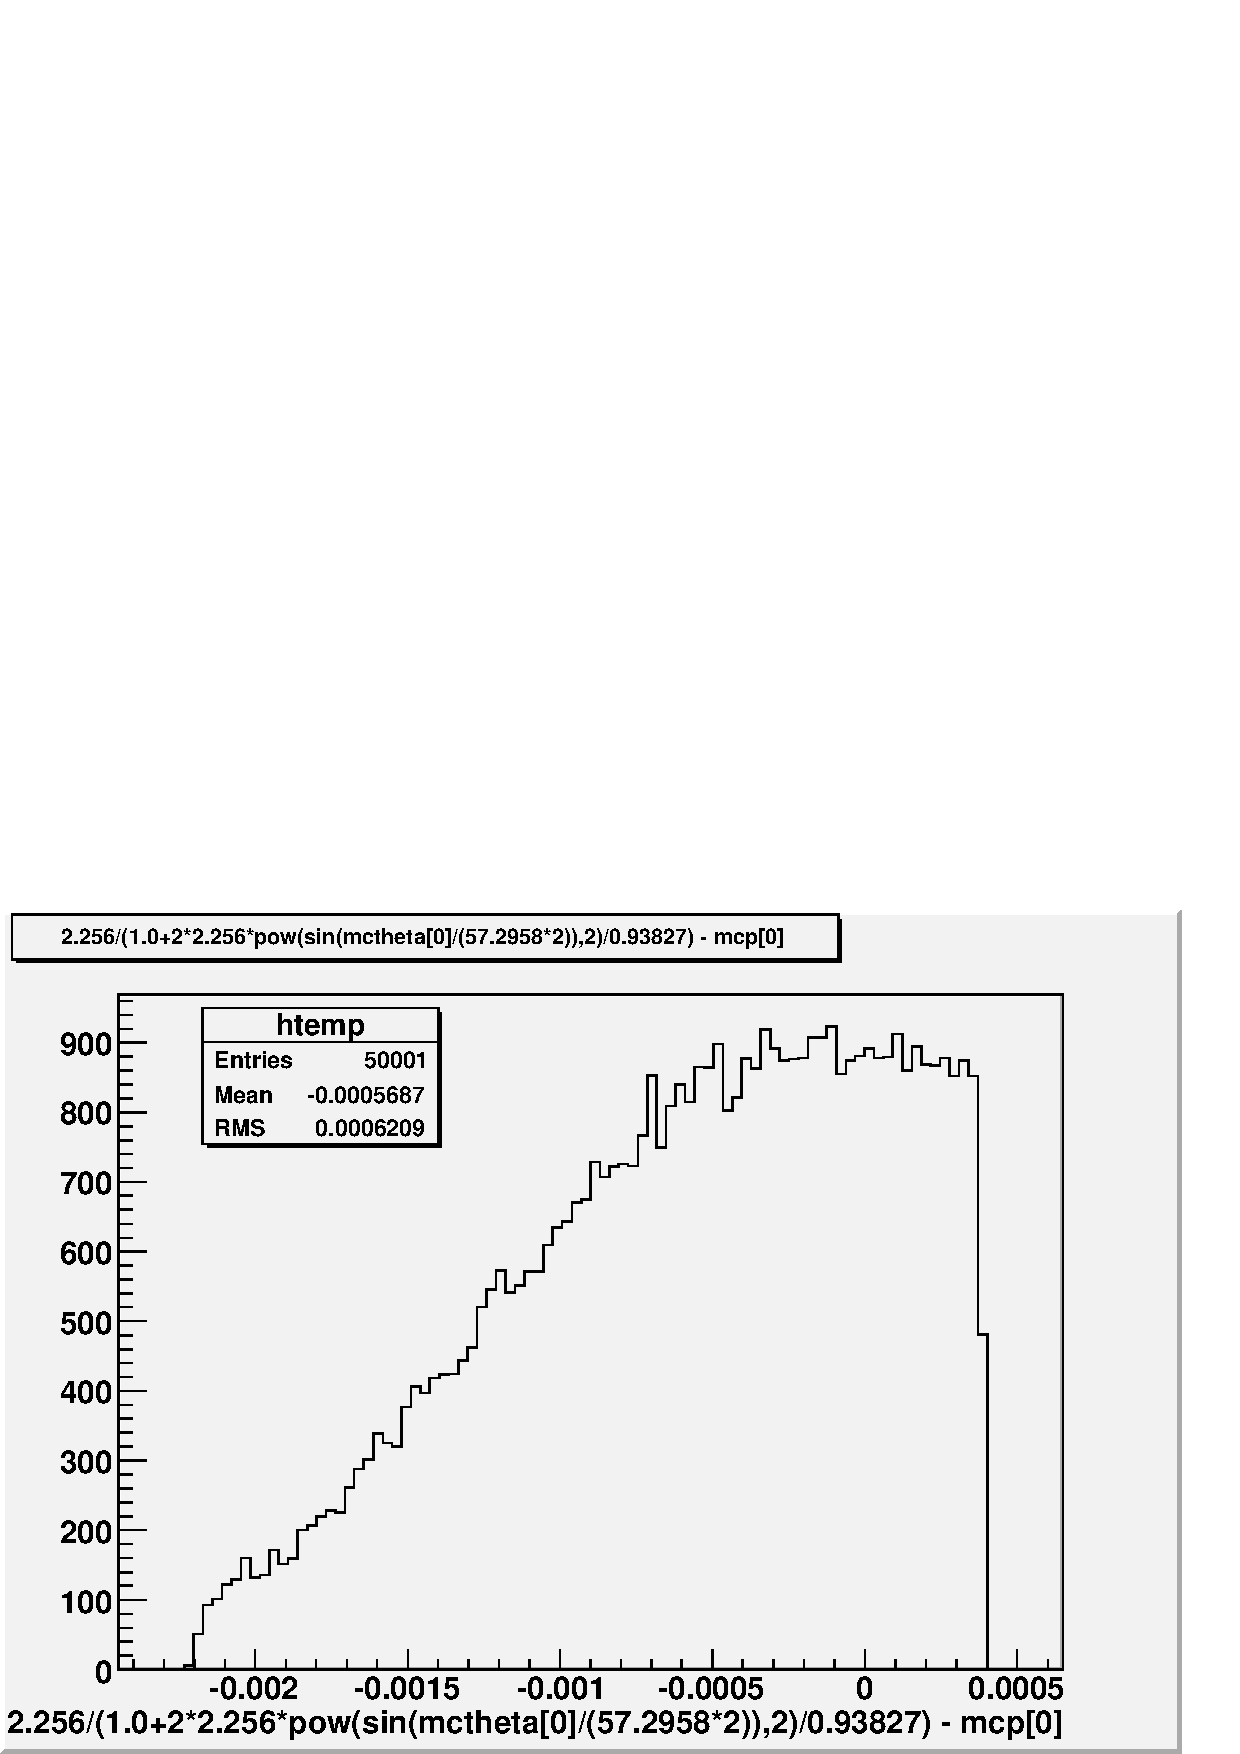
\includegraphics[width=0.6\textwidth]{figuresEG4/DcSmear/genEvntsElastOnlyEb3.png} 
  \caption[$\Delta$E of generated elastic events]{$\Delta$E of 2.3 GeV generated elastic-only proton-target events (no internal radiative effects).}
  \label{fig:genEvnts3}
\end{figure}



\begin{SCfigure} %http://en.wikibooks.org/wiki/LaTeX/Floats,_Figures_and_Captions (needs packages \usepackage[pdftex]{graphicx} & \usepackage{sidecap})
  \centering
  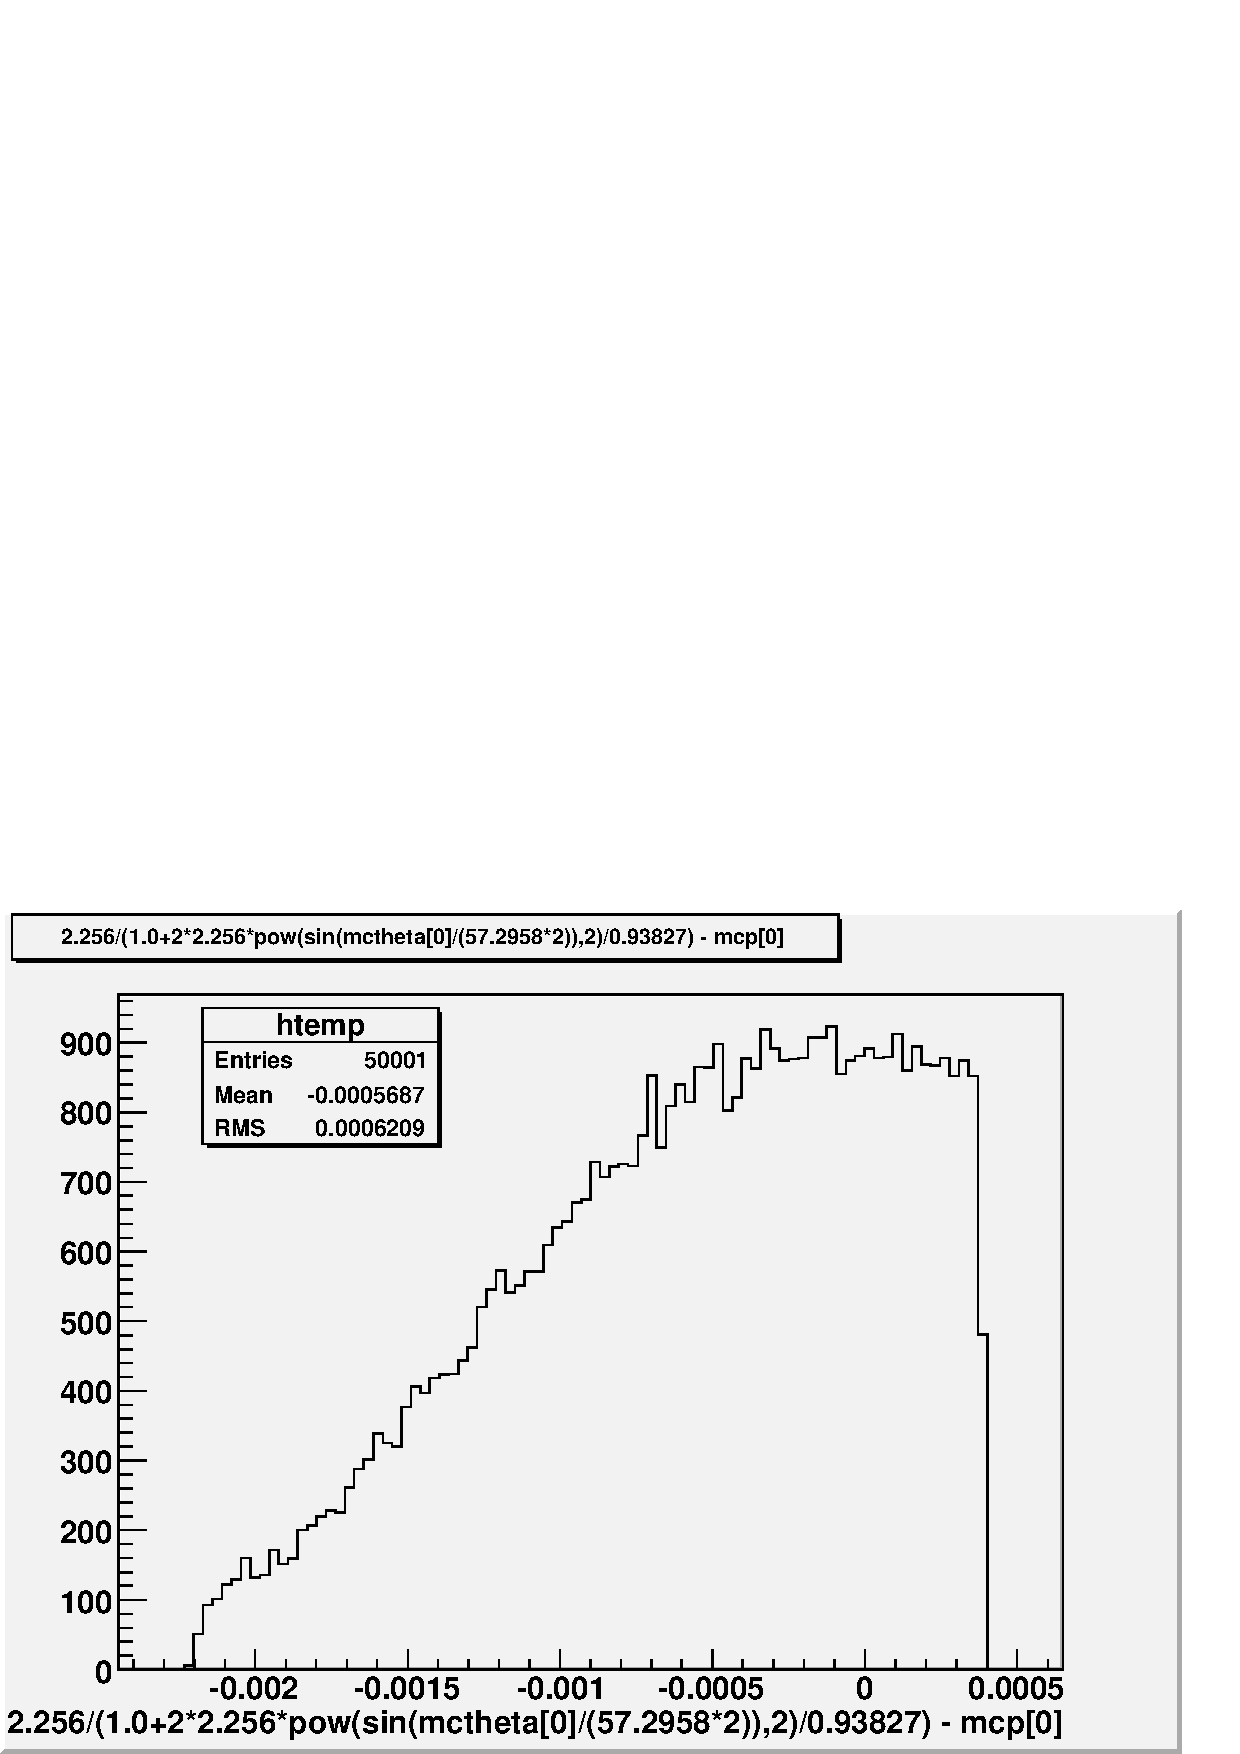
\includegraphics[width=0.7\textwidth]{figuresEG4/DcSmear/genEvntsElastOnlyEb3.png}
  \caption[$\Delta$E of generated elastic events]{$\Delta$E of 2.3 GeV generated elastic-only proton-target events (no internal radiative effects).}
  \label{fig:genEvnts3}
\end{SCfigure}

 \end{comment}

%\subsection{Finding the variation of the width of the simulated elastic peak as a function of DC-smear scale for GPP.}
The simulated elastic events are then fed into GSIM, GPP and RECSIS, with GSIM and RECSIS used in the same configuration as when processing the CLAS data 
during the ``pass-1'' phase, and GPP run with different values of DC-smear scales as inputs. The reconstructed data coming out of RECSIS corresponding to 
a given value of DC-smear is then histogrammed in $\Delta$E again and fitted to a Gaussian to get its $\sigma$ (characterizing width) of and mean 
(characterizing position). As we can see in figures \ref{fig:dcSm1.3} and \ref{fig:dcSm2.9}, %fig(\ref{fig:dcSmEff}), %This didn't give proper number
the width of the elastic peak increases with the DC-smear but the position stays more or less the same as expected. In fact, when the two are plotted 
against DC-smear (as in figures \ref{fig:SigmaVsm} and \ref{fig:MeanVsm}) %(as in fig (\ref{fig:ParsVsm})), %This didn't give proper number 
the width shows a linear dependance.



%Don't delete the following commented out lines. They are important reminders.
%The following four images are made using ~/Acceptance/SimStuffs/dE_resolHistoFits.C and enabling ``#define DRAW_EPS'' & ``#define USE_THETA_ALL''
\begin{comment} %=======================================Comments begin
%idea source: http://texblog.wordpress.com/2007/08/01/placing-figurestables-side-by-side-minipage/ : Placing figures/tables side-by-side (\minipage)
%This method of putting figures/tables side by side doesn't have the option of global caption (if there is, it treats it like a
% caption of a different figure assigning it with a different figure number in the output file. So, I chose the 'subfigure' method instead
\begin{figure}[h]
\begin{minipage}[b]{0.5\linewidth}
\centering
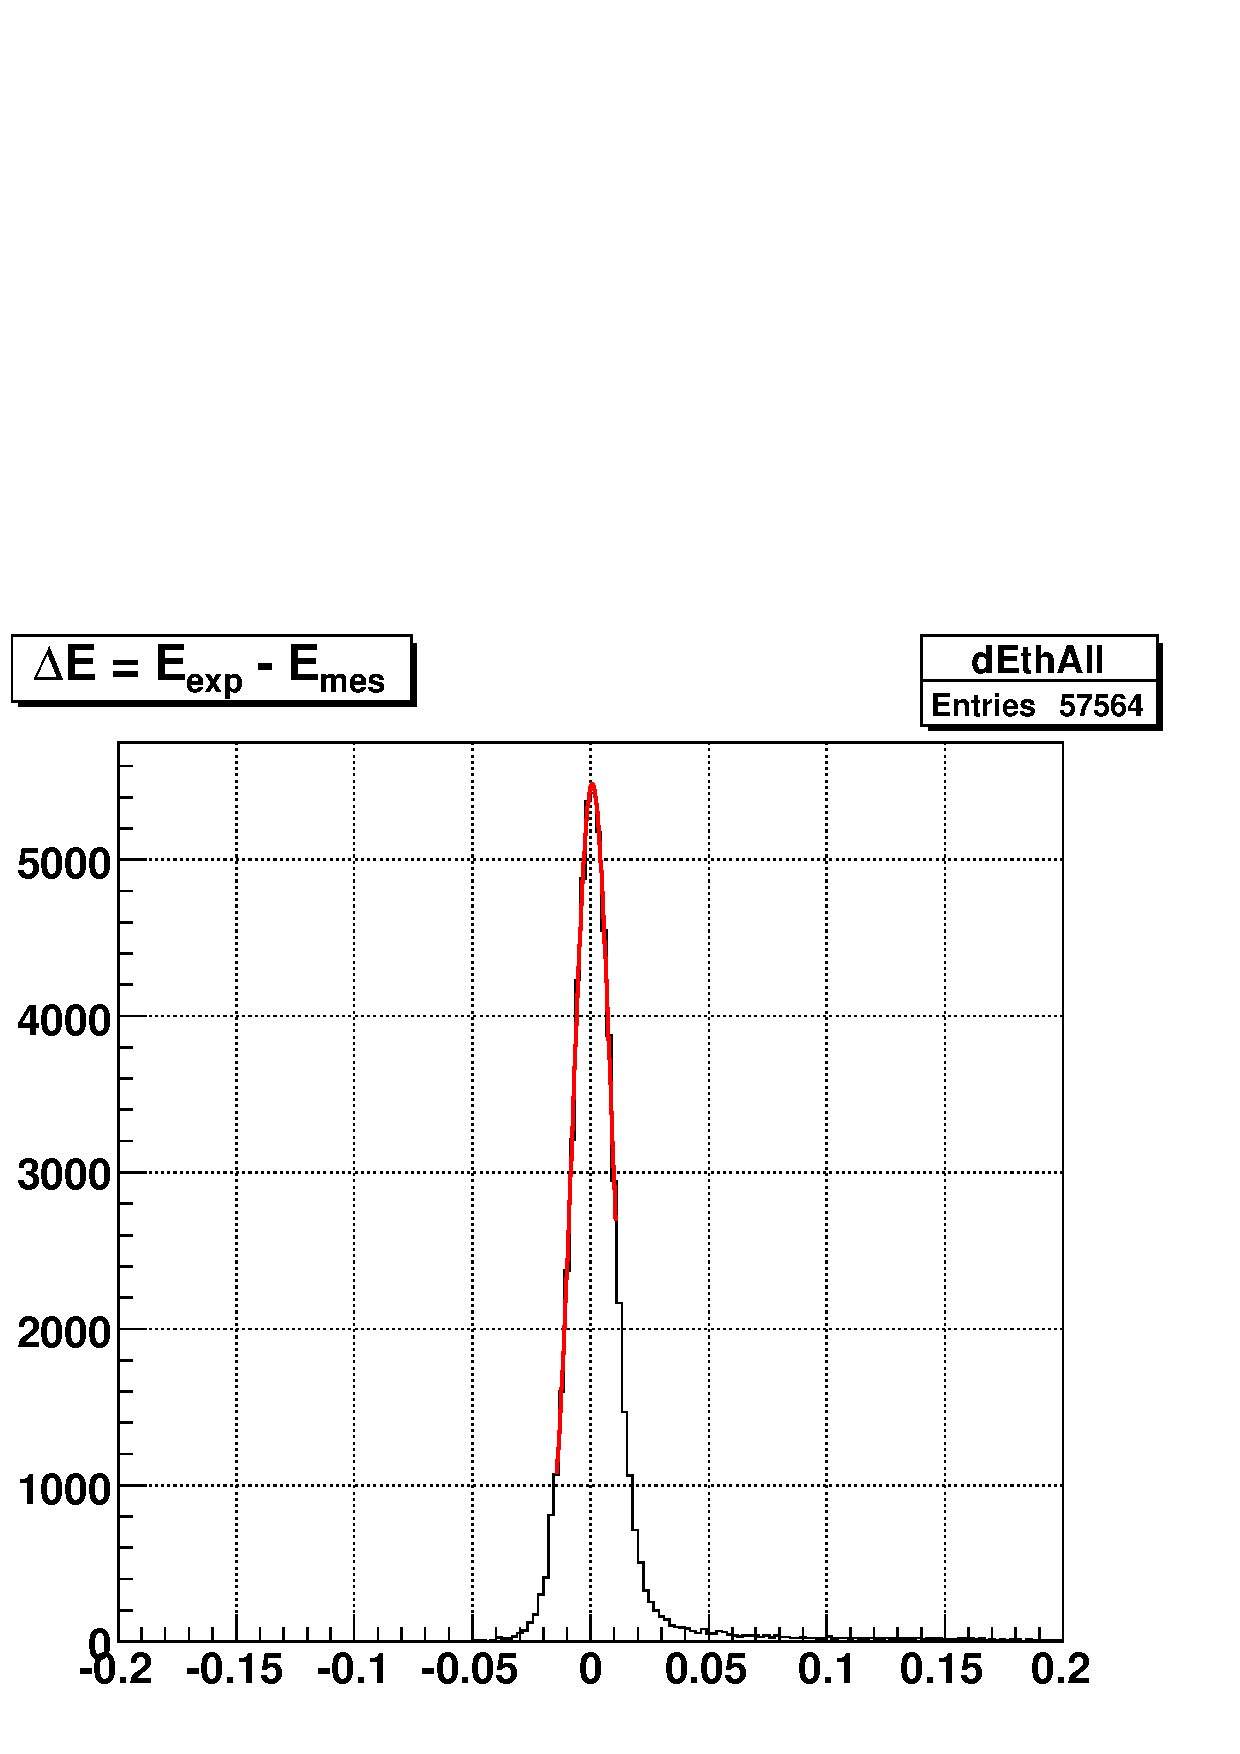
\includegraphics[scale=0.37]{figuresEG4/DcSmear/dE_ThAllEb3_DcSmear1.3.png}
\caption{$\Delta$E of 2.3 GeV simulated elastic-only proton-target events (see fig(\ref{fig:genEvnts3})) after passing through GSIM, GPP 
  (with Dc-smear scale of 1.3) and RECSIS.}
\label{fig:figure1}
\end{minipage}
\hspace{0.0cm} %\hspace{0.1cm}
\begin{minipage}[b]{0.5\linewidth}
\centering
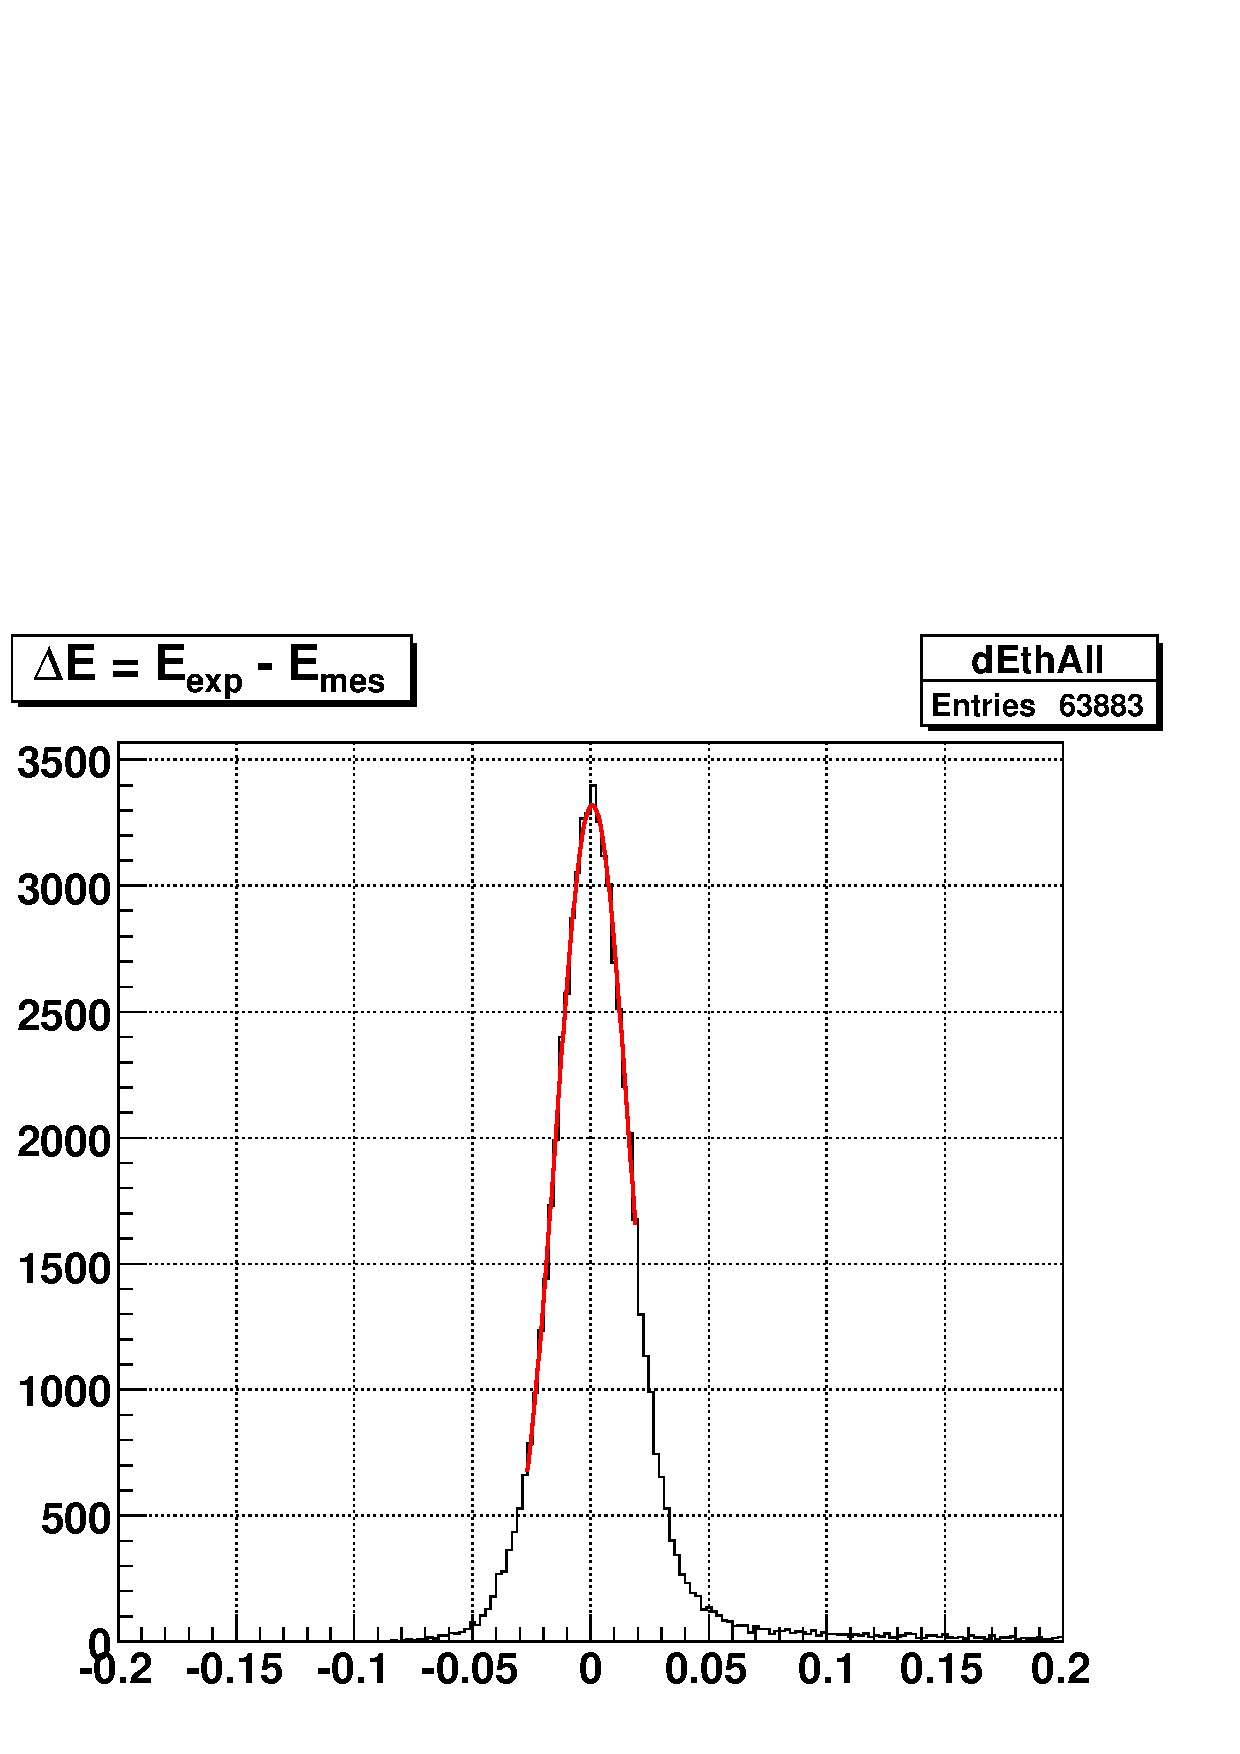
\includegraphics[scale=0.37]{figuresEG4/DcSmear/dE_ThAllEb3_DcSmear2.9.png}
\caption{$\Delta$E of 2.3 GeV simulated proton elastic-only events after passing through GSIM, GPP (with Dc-smear scale of 2.9) and RECSIS.}
\label{fig:figure2}
\end{minipage}
\caption{$\Delta$E of 2.3 GeV simulated elastic-only proton-target events (see fig(\ref{fig:genEvnts3})) after passing through GSIM, GPP (with Dc-smear scale of 1.3) and RECSIS.}
\end{figure}
\end{comment}  %=======================================Comments end


% idea source: http://texblog.wordpress.com/2007/08/28/placing-figurestables-side-by-side-subfigure/ :Placing figures/tables side-by-side (\subfigure)
% Can include any number of figures/tables, not just two.
\begin{figure}[H]
\centering
\subfigure[Dc-smear]{
\includegraphics[scale=0.32]{figuresEG4/DcSmear/dE_ThAllEb3_DcSmear1p3}%.png}
\label{fig:dcSm1.3}
}
\subfigure[Dc-smear]{
\includegraphics[scale=0.32]{figuresEG4/DcSmear/dE_ThAllEb3_DcSmear2p9}%.png}
\label{fig:dcSm2.9}
}
\label{fig:dcSmEff} %Effect of Dc-smear
%\caption[Optional caption for list of figures]{Caption of subfigures \subref{fig:subfig1}, \subref{fig:subfig2} and \subref{fig:subfig3}}
\caption[$\Delta$E of reconstructed simulated events]{$\Delta$E of 2.3 GeV simulated elastic-only proton-target events passing through GSIM, GPP (with two different Dc-smear scales), and RECSIS.}
\end{figure}




\begin{figure}[H]
\centering
\subfigure[$\sigma$ vs DC-smear]{
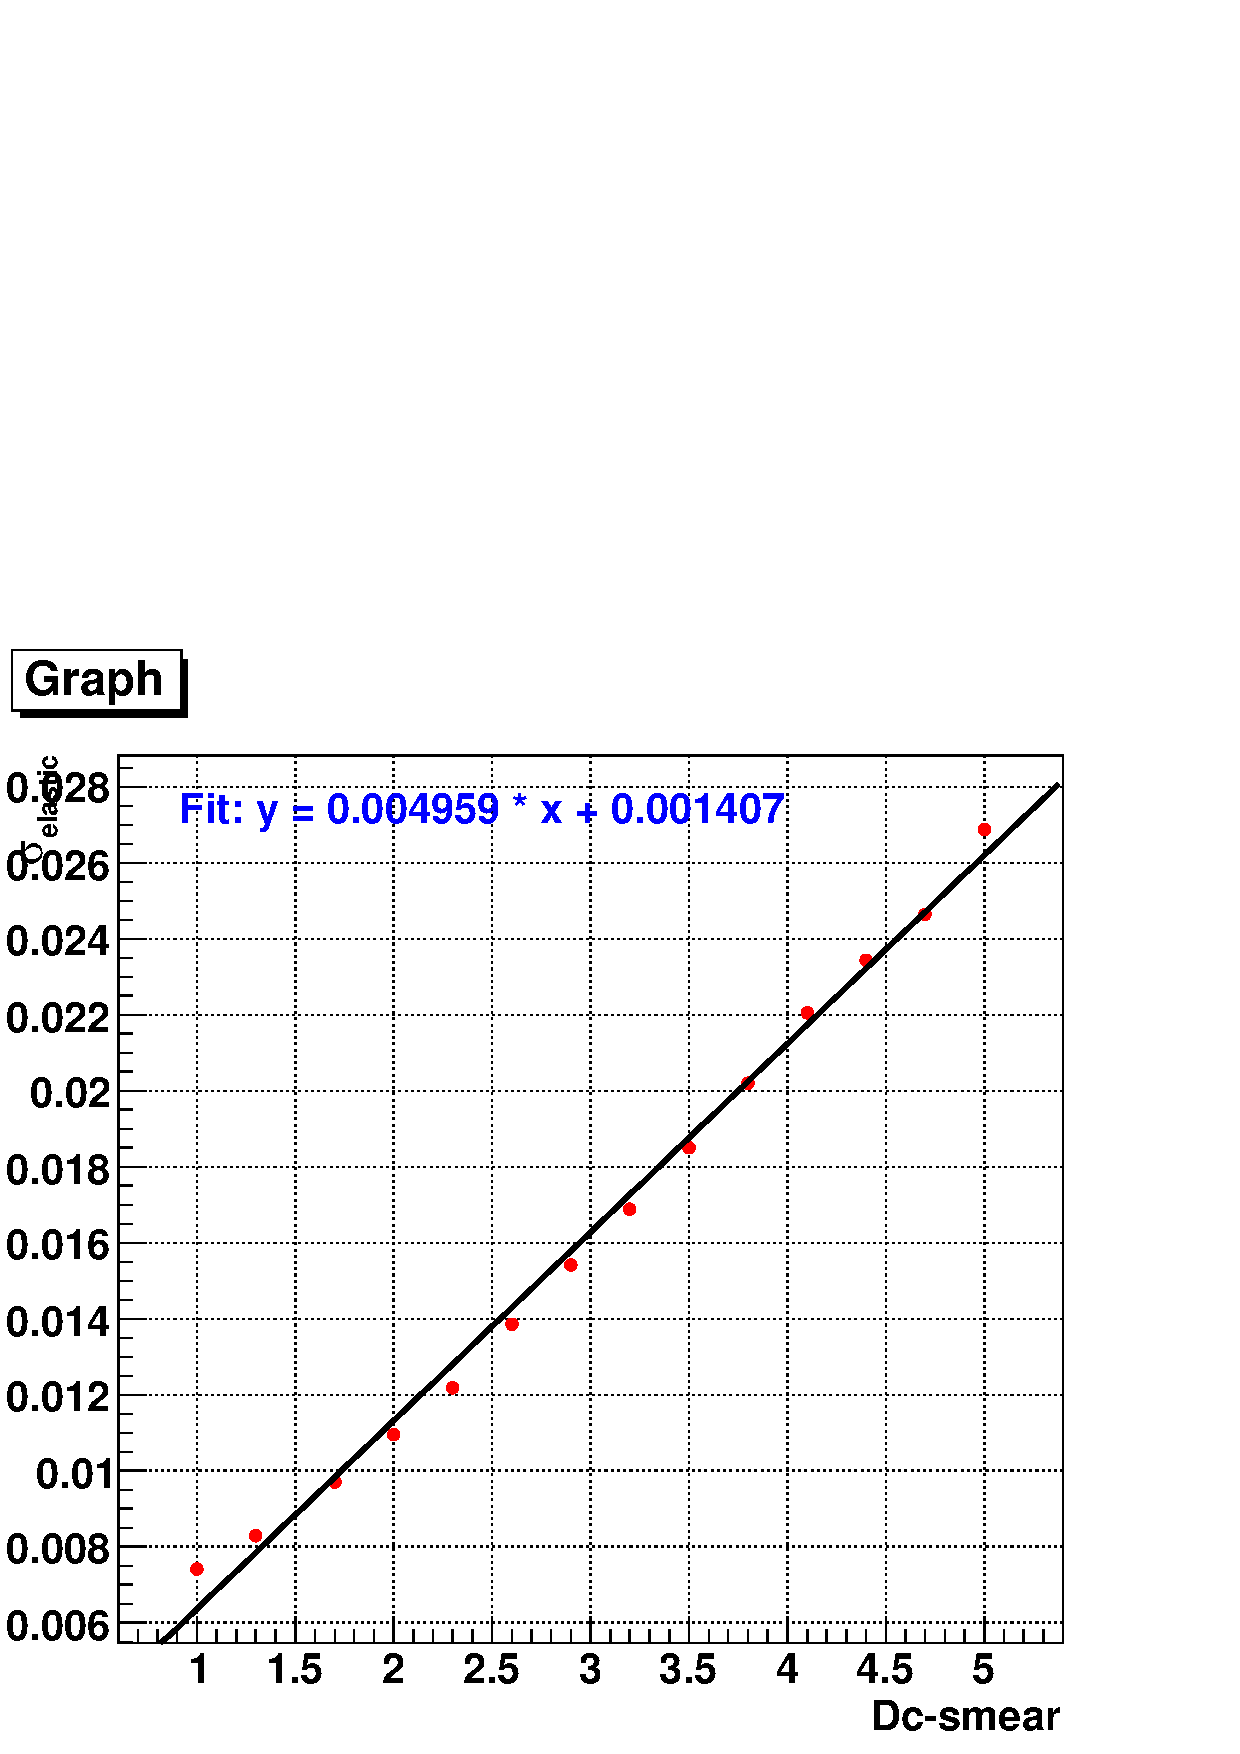
\includegraphics[scale=0.32]{figuresEG4/DcSmear/grSigmaVsDcSmear_Eb3.png}
\label{fig:SigmaVsm}
}
\subfigure[Mean vs DC-smear]{
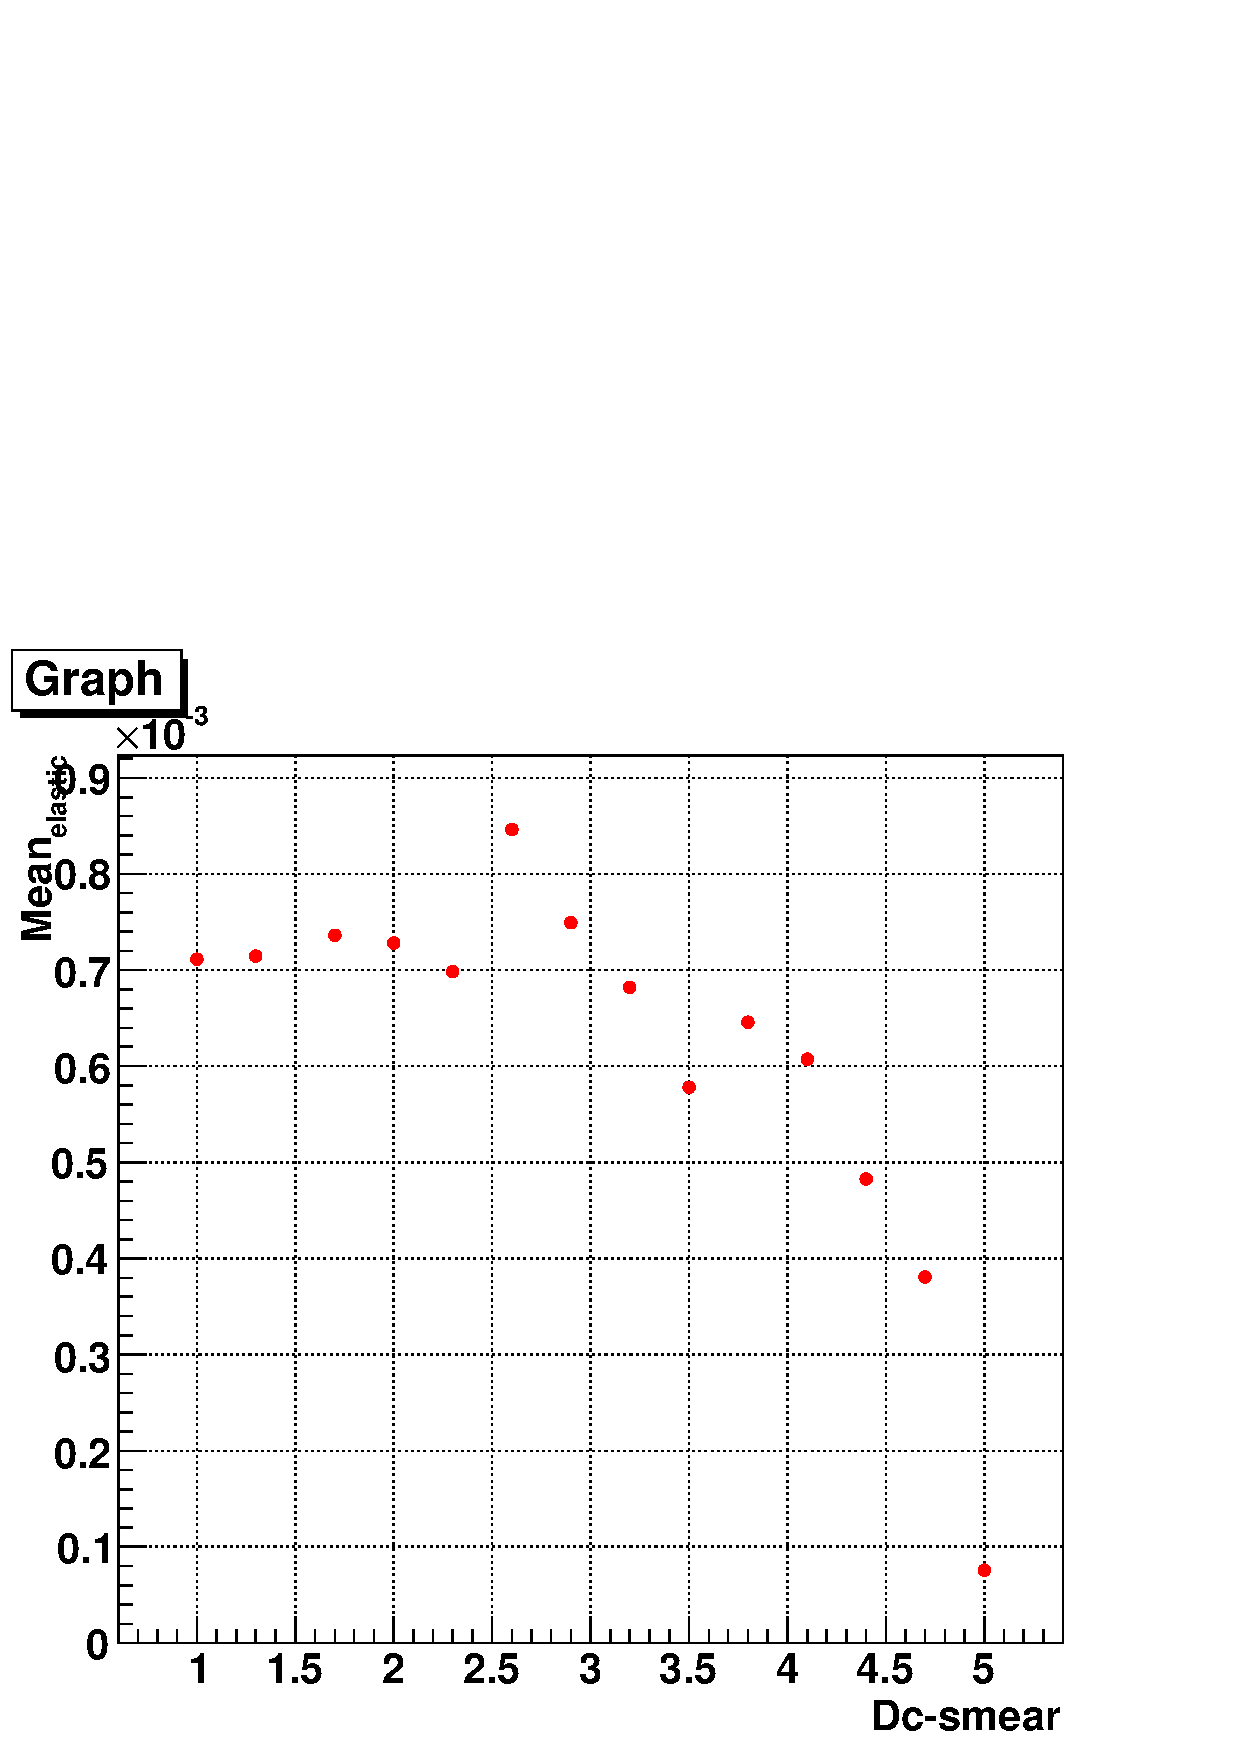
\includegraphics[scale=0.32]{figuresEG4/DcSmear/grMeanVsDcSmear_Eb3.png}
\label{fig:MeanVsm}
}
\label{fig:ParsVsm} %Effect of Dc-smear
%\caption[Optional caption for list of figures]{Caption of subfigures \subref{fig:subfig1}, \subref{fig:subfig2} and \subref{fig:subfig3}}
\caption[DC-smearing effects on elastic peak]{Graphs showing the dependence of width and position (obtained from the Gaussian fits as shown in the fig (\ref{fig:dcSmEff}) of the elastic peaks on the DC-smear applied to GPP.}
\end{figure}


\subsection{Finding the width of the real CLAS data elastic peak.}
With the knowledge of the DC-smear dependence of energy resolution (Fig. \ref{fig:SigmaVsm}), if we also know the resolution in the real data, 
we can determine the right value of DC-smear which would make the resolution in the simulation comparable with that in the real data. So, 
the next step is to find the resolution in the real CLAS data, which is done again by measuring the width of the elastic peak in the real data. 
But, because the real data is a very complex mixture of events coming from various reaction channels, we must first have a way to separate the elastic 
data from the rest. One method entails histogramming \dE from both the \nh3 and \c12 target data (for a given beam energy) and subtracting 
the latter (after the cross-normalization) from the former (as in fig (\ref{fig:elNH3mC})) to effectively remove the contribution from nitrogen 
component of the \nh3 target leaving the contribution coming only (mostly) 
%More words about this background subtraction can be found in the section for the inclusive momentum correction.
from the proton component. Another method consists of using only the \nh3 data but this time calculating the helicity dependent cross-section 
difference in the elastic region Fig. (\ref{fig:elXsDif}). In the latter method, the difference removes the contribution from the unpolarized 
nuclear background because they have the same contribution to the opposite helicity state cross-sections. After the elastic data is separated, its 
\dE distribution is fitted to a Gaussian as with the simulation data and we arrive at the experimental energy resolution. 
%Since on the simulation side, we used the total cross-section, to make an apple-to-apple comparison, the measurement coming from the 1st method
%would be better choice for the experimental data.

% Put a intra-thesis chapter/section link (rather than the web link) in thesis version
% \href{http://www.jlab.org/Hall-B/secure/eg4/ripani/Reference/Reference.html}{groups 1, 2 and 4 cuts}. 
% Check DoEvent..() function in file /u/home/adhikari/Acceptance/SimStuffs/dE_resol_DataSim.C to see what cuts were used to select the events


%The following image is made using ~/Acceptance/SimStuffs/subtractHistos4ProdElast.C and enabling ``#define DRAW_EPS'' & ``#define USE_THETA_ALL''
%The following four images are made using ~/Acceptance/SimStuffs/dE_resolHistoFits.C and enabling ``#define DRAW_EPS'' & ``#define USE_THETA_ALL''
\begin{figure}[h] %ht, htpb (p - float, b = bottom, h=? t = top)
\centering
  \leavevmode 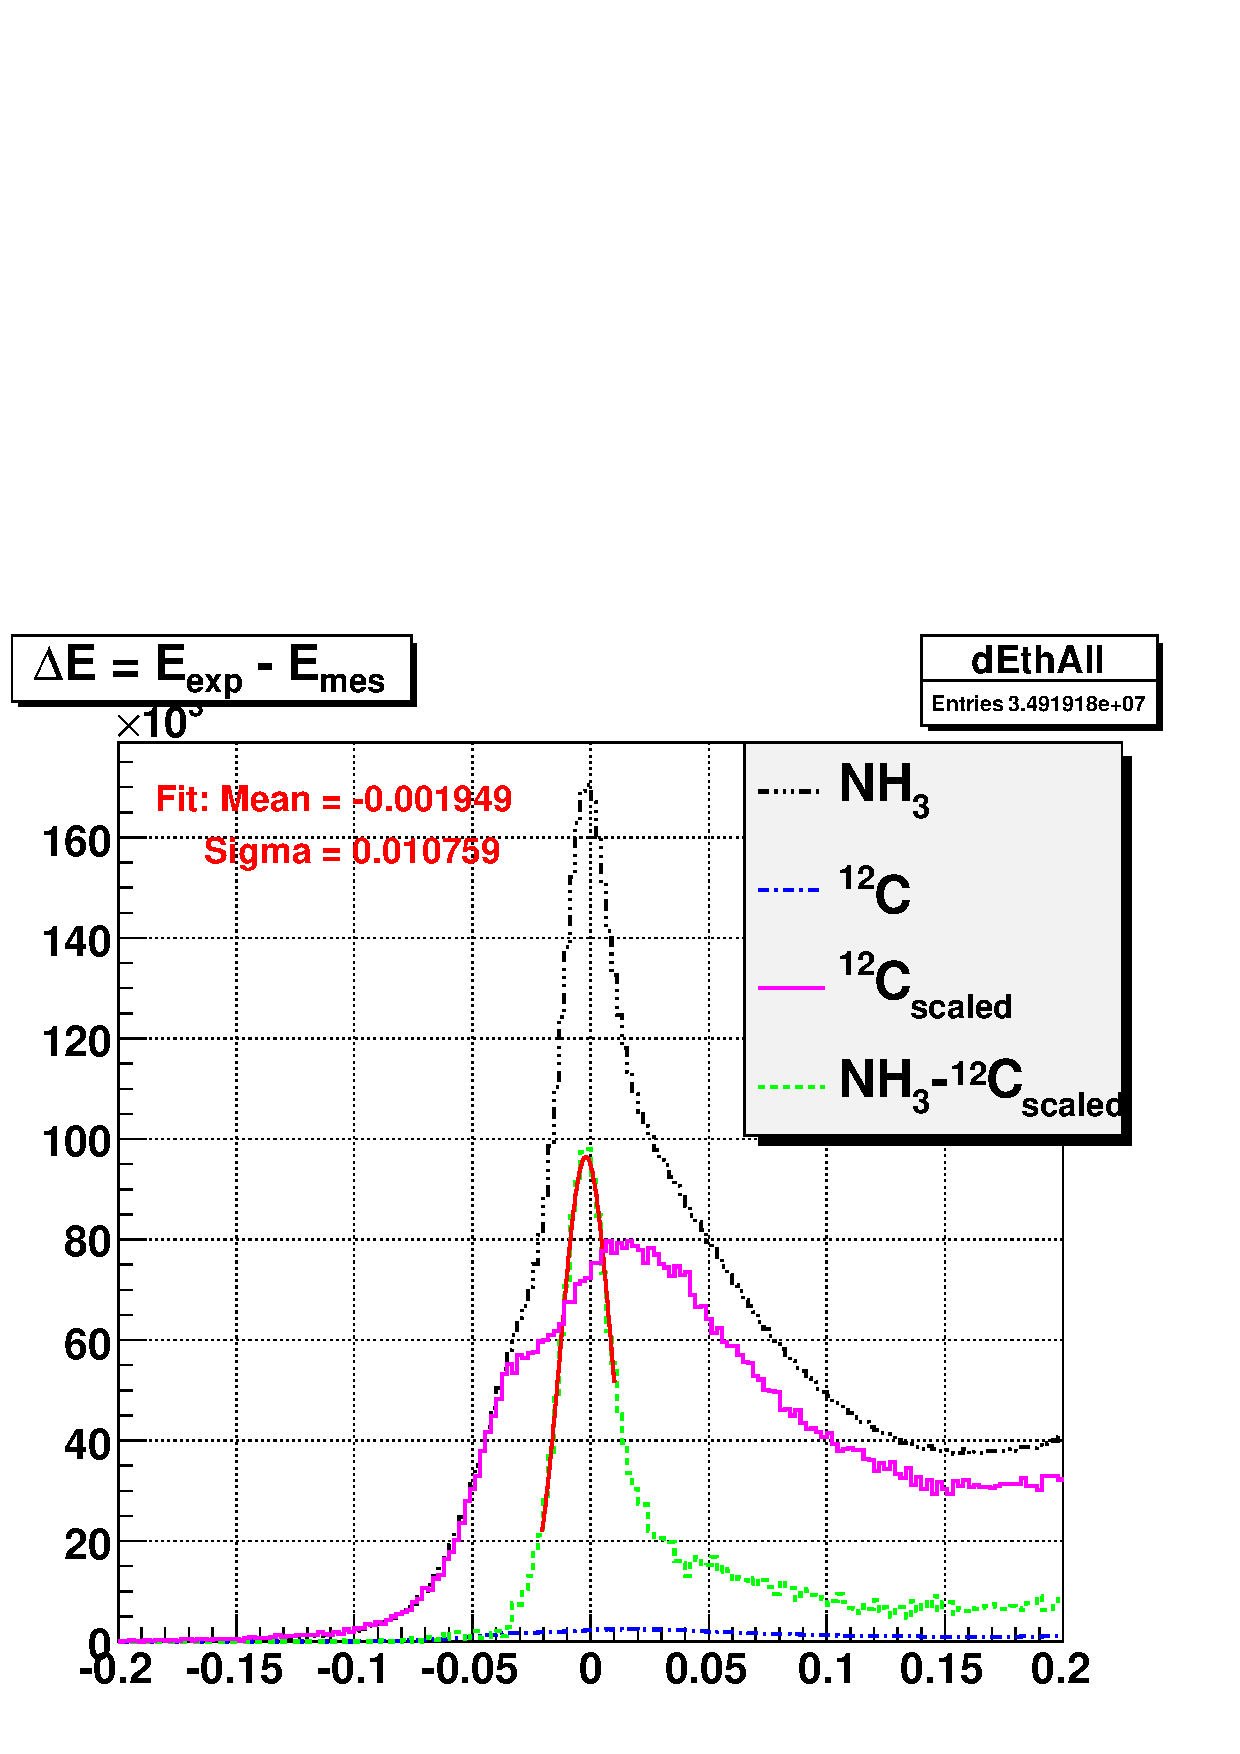
\includegraphics[width=0.8\textwidth]{figuresEG4/DcSmear/dE_elastProdEb3.png} 
  \caption[Background subtraction to get elastic peak]{Histograms illustrating the extraction of elastic peak for 2.3 GeV by using carbon-12 data for background removal from the total-cross section (all good electrons with $\theta>7$ used).}
  \label{fig:elNH3mC}
\end{figure}

%The following image is made using ~/Acceptance/SimStuffs/subtractHistos4xsDiff.C and enabling ``#define DRAW_EPS'' & ``#define USE_THETA_ALL''
\begin{figure}[h] %ht, htpb (p - float, b = bottom, h=? t = top)
\centering
  \leavevmode 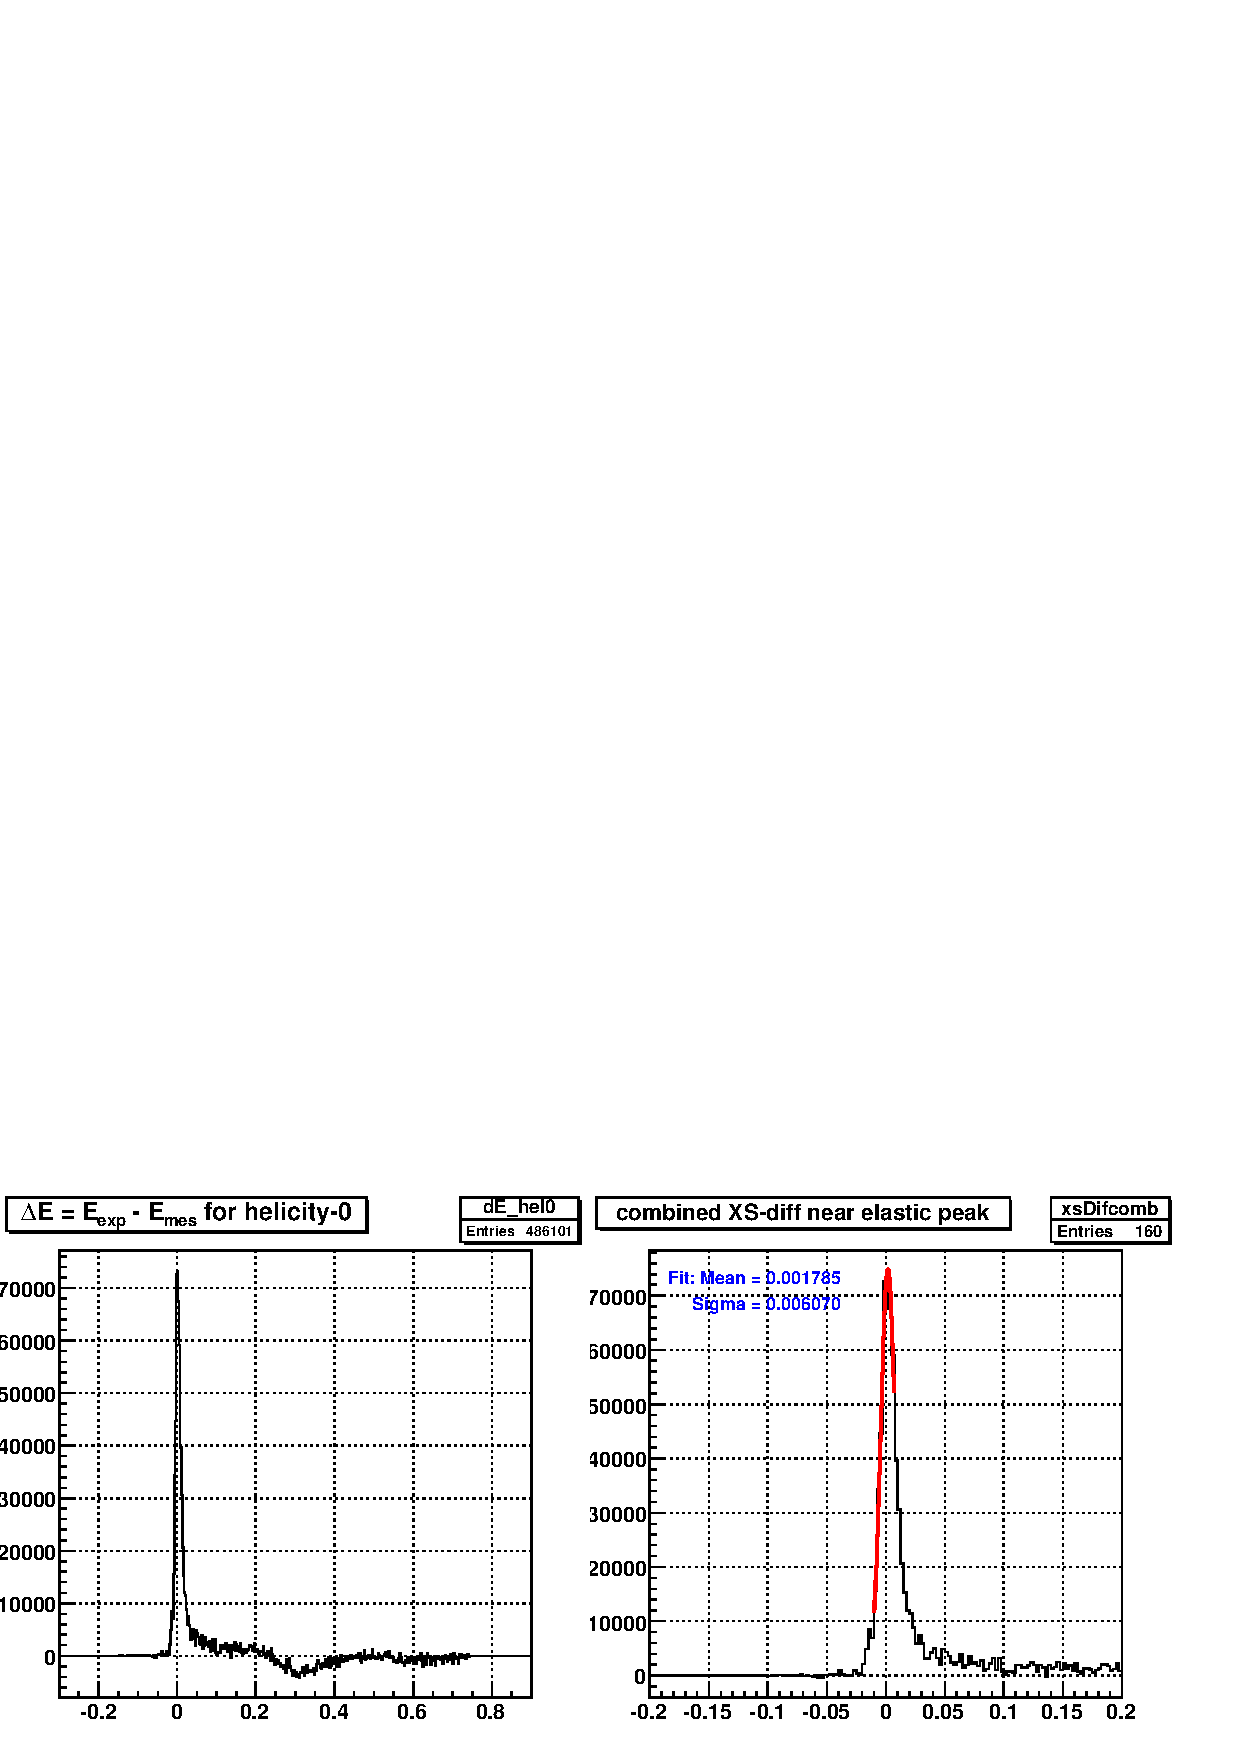
\includegraphics[width=1.0\textwidth]{figuresEG4/DcSmear/dE_elastXsDiffEb0Tgt11.png} 
  \caption[Cross-section difference]{Plots showing the cross-section difference for 2.3 GeV NH$_3$ target data with the right one zoomed in around the elastic region (all good electrons with $\theta>7$ used).}
  \label{fig:elXsDif}
\end{figure}

 %\\ %12/4/13 (Addressing Gabriel's concern)
 %\\
 



%\subsection{Comparing the width of the real CLAS data elastic peak and those from Simulation with different DC-smears.}
%The following two images are made using ~/Acceptance/SimStuffs/graphSigmaVsEb.C and enabling ``#define DRAW_EPS'' & ``#define USE_THETA_ALL''
Using the first of the two methods mentioned above, the real data resolutions were evaluated for three different %cases 
polar angle ($\theta$) cuts - 
all \th (in fact $\theta\ge7^o$), $\theta>15^o$, and $\theta>20^o$. The dependence of these experimental resolutions on the beam energy for these cases are 
shown together in the Fig. \ref{fig:sigsProd}, along with the resolution for the case ``all $\theta$'', but determined from the cross-section difference 
method. Likewise, as described above, the DC-smear dependence of the simulated resolution were determined separately for all these three cases of 
angle cuts, so that we could compare the experimental resolutions with the simulations correspondingly. One such comparison is illustrated in 
the figure \ref{fig:sigsProdSim}, where we show resolutions evaluated for the case of ``all \th'' - first two for the experimental data and the rest for 
the simulated data. 

    
     
 \begin{figure}[h] %ht, htpb (p - float, b = bottom, h=? t = top)
\centering
  \leavevmode \includegraphics[width=1.0\textwidth]{figuresEG4/DcSmear/graphSigmaVsEb_prodOnly.png} 
  \caption[$E_{beam}$ dependence of DC smearing (Experimental) ]{Graphs showing the dependence of width ($\sigma$) of the elastic peaks (from experimental data) on the beam energy (GeV).}
  \label{fig:sigsProd}
\end{figure}
    
 \begin{figure}[h] %ht, htpb (p - float, b = bottom, h=? t = top)
\centering
  \leavevmode 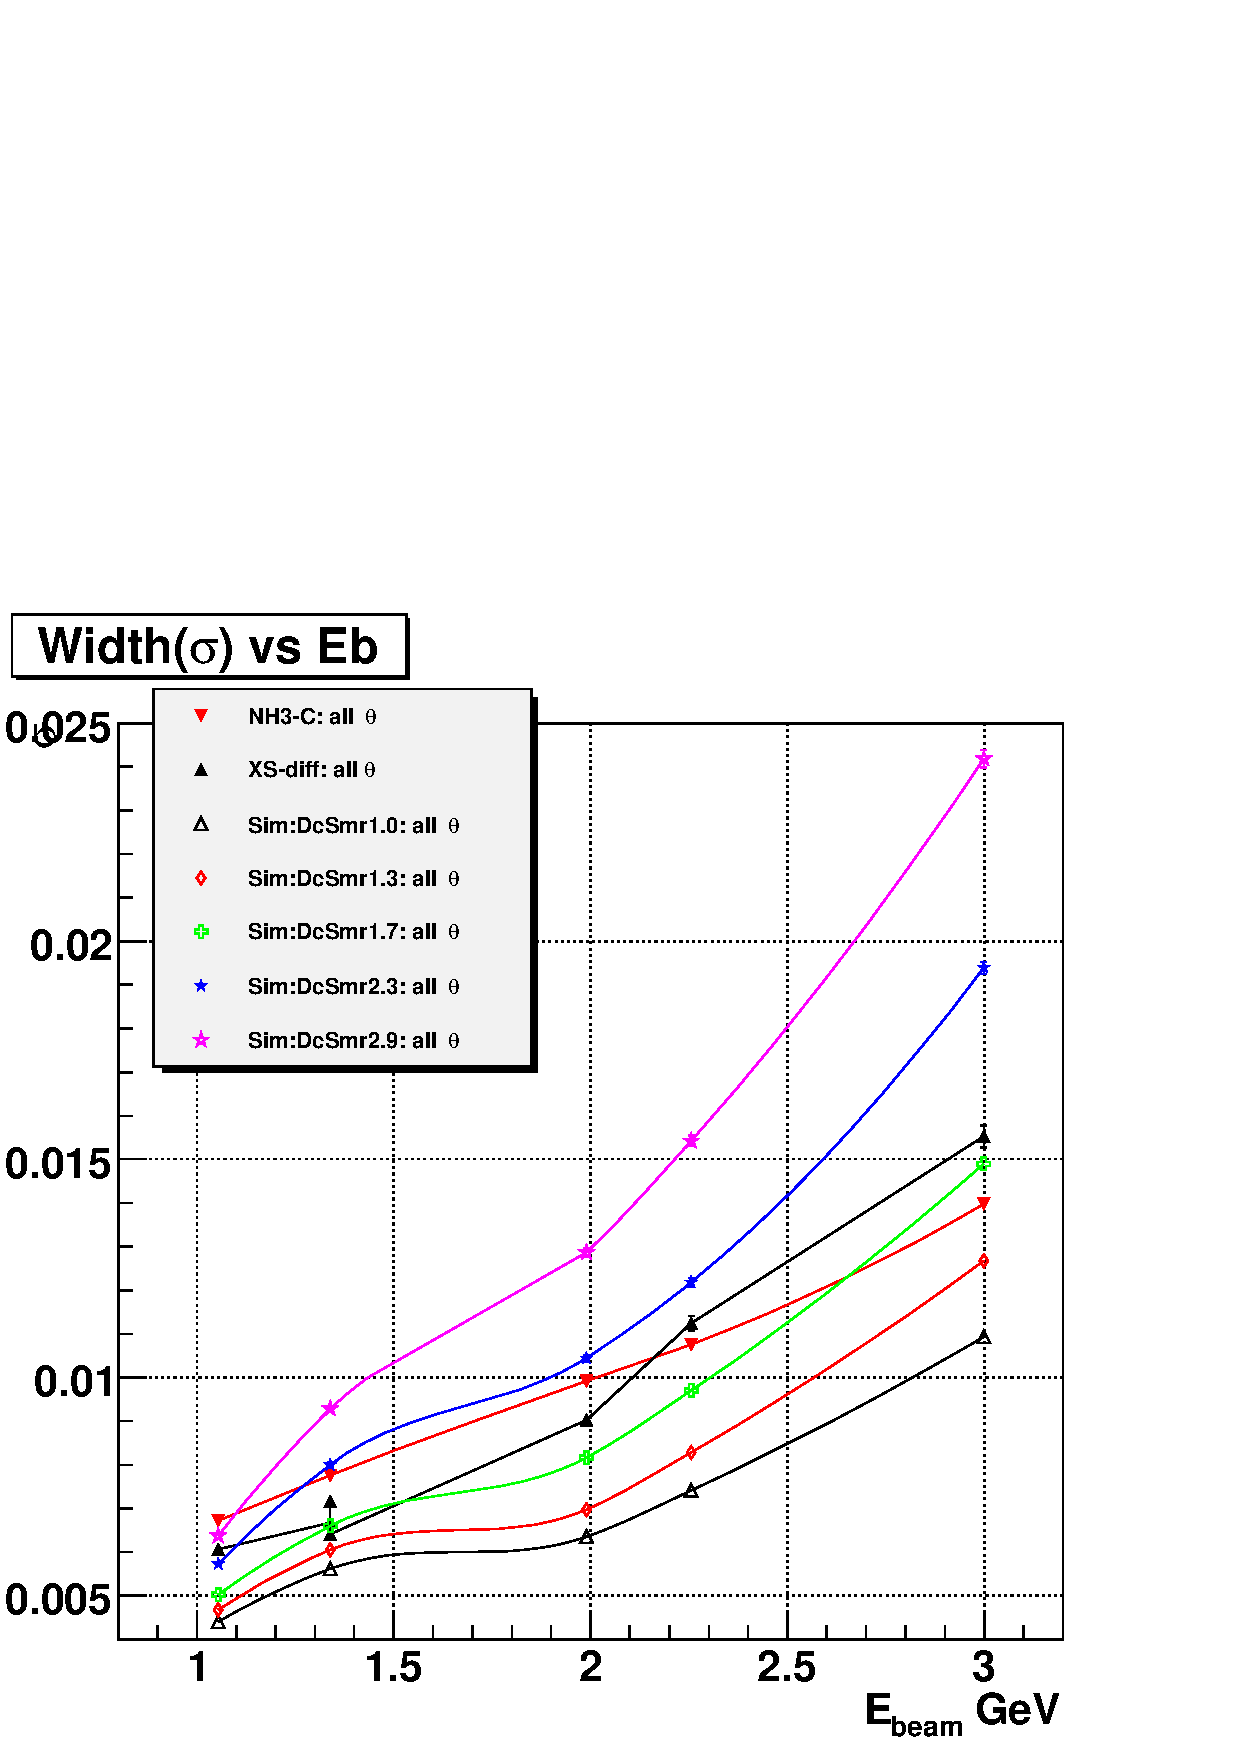
\includegraphics[width=1.0\textwidth]{figuresEG4/DcSmear/graphSigmaVsEb_SimThAll.png} 
  \caption[$E_{beam}$ dependence of DC smearing (Experimental) ]{Graphs showing the dependence of width ($\sigma$) of the elastic peaks (from both experimental and simulated data) on the beam energy (GeV).}
  \label{fig:sigsProdSim}
\end{figure}
    
     
     
Looking at Fig. \ref{fig:sigsProd}, it is obvious that the resolution is $\theta$-dependent as expected. %Remember resol = beta/sqrt(p_t), mom-cor
When the experimental and simulated resolutions are compared for the three different cases of $\theta$ cuts, we realize that the GPP asks for the 
\th dependent DC-smearing, which makes the simulation work very complicated with the current version of GPP. To simplify the situation, we decide to 
have a global (\th independent) value of DC-smearing (for a given beam energy) by comparing the experimental and simulated resolutions corresponding to 
the case of ``all \th'' cut. %That should be good enough for practical purposes. %xz:
%xz: "That should be good enough for practical purposes". Why?  Be careful to never make a statement without backing it up.
By taking into account the fact that there seems to be an inherent 
uncertainty in the measurement of the resolutions (evident from the discrepancy of the experimental resolutions determined from the two different methods)
and comparing the experimental and simulated results, the values as listed in Table. \ref{tab:dcSmears} are chosen for the DC-smearing scales for the GPP.


%\FloatBarrier  
% \FloatBarrier %http://tex.stackexchange.com/questions/9485/how-to-fix-table-position
%\begin{center}
\begin{table}[H]%[h] %[h!b!p!]
\centering
    \caption{DC-smearing scales determined for different beam energies.}
    \label{tab:dcSmears}
    \begin{tabular}{ | l | l | l | l | l | l |}
    \hline
    $E_{beam}$ (GeV) & 1.054  & 1.339 & 1.989 & 2.256 & 2.999 \\ \hline
    DC-smear         & 2.6    & 2.0   & 2.0   & 2.0   & 1.7 \\  \hline
    \end{tabular}
%    \caption{DC-smearing scales determined for different beam energies.}
%    \label{tab:dcSmears}
\end{table}
%\end{center}




\begin{comment} %==================My comments on the generated events==========Comments begin=== Sep 19, 2011
%The events were generated by using the Genova inherited mod_osip_bost (aka STEG) generator 
      subroutine smrad_proton(Es,theta,Ep,sig_el,sig_tot,sel,smin)
      common/material/TG
      sn2=(sin(theta/2.0))**2     Q2=4.0*Es*Ep*sn2       nu=Es-Ep
c-----input values
      Mp=0.93827        Z=1      A=1     E3=Es/(1.0+Es*(1.0-cos(theta))/Mp)
c-----elastic peak width==resolution
      dWp=0.001       delta_E=(dWp+dWp**2/(2.0*Mp))/(1.0+2.0*Es/Mp*sn2)/5.
c-----Target thickness
      t=0.0181              ! 0.6 cm NH3
      tiw=0.0079            ! 7.45 mm He
      tfw=0.0079            ! 7.45 mm He

      elra=0.0d+0       innn=0.0d+0       eltail=0.0d+0
c-----cross section
      if(Ep.gt.(E3-2.0*delta_E)) then
      varr=abs(nu-Q2/(2.0*Mp))
      jack=Es/E3
      elcor=elasrad_proton(Es,theta,t,delta_E,Z,A,tiw,tfw)                     ! cole smith program for radiative correction in the elastic region
      elra=sig_elastic_proton(Es,theta,Mp,Z)*elcor*peak_proton(varr,dWp)*jack
      
      innn=0.0d+0
      eltail=0.0d+0
      else
      elra=0.0d+0
      
      streg_tail=straggling_elasic_proton(Z,Mp,t,Es,Ep,theta,delta_E)           !But this is not added to anything so it's inconsequencial
      endif
            
      sel=elra+eltail
      smin=elra+innn+eltail
      return
      END


Comments:
There are two if blocks in the above chunk of the code:
     a) the ``if'' block which covers the elastic region
     b) the  ``else'' block which covers the rest of the region.
The else block has zero contribution to the value returned by the function because we set 'innn' and 'eltail' to zero and 'streg_tail' is not added to 
the sum to be returned.

As we see, the way I did is (being unsure how to turn off the effect of elcor (Cole smith's rad-corr)) leave the target widths t, tiw and tfw as they 
were (i.e. to non-zero values), and also leave the elcor factor alone, so that it would have some modulating effect on the remaining part of the product  
i.e. sig_elastic_proton(Es,theta,Mp,Z)*peak_proton(varr,dWp)*jack. Initially I thought I would give elcor an artificial value of 1.0 and that would 
probably turn off the effect. But, because of lack of confidence in that idea, I abandoned that idea and left it to modulate the elastic peak (may be 
the peak would come out more like a Gaussian, if I had done that). Even with that modulation, the generated events are within 3 MeV range and so the 
modulation would be insignificant. Another thought that came to my mind was that since this factor should have the effect of reducing the events in the 
elastic region to compensate for the radiative tail that we get beyond the elastic region, and since we're not simulating that part, there is no point 
in worrying about that reduction. If if the factor reduced the cross-section, the generator would produce the same number of events by running some extra 
mile to compensate for that reduction. 
\end{comment}  %=======================================Comments end
    % Disabled



%\subsection{RECSIS - Event Reconstruction}
%\label{recsis}
%\textbf{\textcolor{red}{Comment: Similar discussion on RECSIS may come elsewhere too, because RECSIS is used in the experimental data reconstruction too, so the section here may simply refer/cite that section rather than re-inventing the wheel.}}\\ %\\%\newline
%\textbf{Elaborate more on corrections.}
% Zixie thes: pg71, Nevzat: pg 111, 

%These GPP output that has the detector signals in response to the Monte Carlo events are then fed through  RECSIS (which processes them the same way as real data) to reconstruct the passed events.





